\documentclass[12pt]{article}
\usepackage[bottom = 3cm, left = 3cm, right = 3cm, top = 3cm]{geometry}
\usepackage{amssymb}
\usepackage{graphicx} % Required for inserting images
\usepackage{caption}
\usepackage{tikz}
\usepackage{url}
\usepackage{amsmath}
\usepackage[colorlinks]{hyperref}
\usepackage{graphicx}
\usepackage{subcaption}

%Bibliography
\bibliographystyle{plain}
\usepackage{biblatex}
\addbibresource{bibliography.bib}


\DeclareUnicodeCharacter{2212}{\ensuremath{-}} %To avoid some error with the - symbol

\begin{document}


\begin{titlepage}
    \begin{center}
        \vspace*{1cm}
            
        \Huge
        \textbf{Student Visit Report}
            
        \vspace{0.5cm}
        \LARGE
        Thin Liquid Films, Numerical Simulation and Control
            
        \vspace{1.5cm}
            
        Bilal Ben Moussa
            
        \vfill
            
        With the Supervision of \\
        Dr.Susana Gomes \& Dr.Radu Cimpeanu
            
        \vspace{0.8cm}
            
        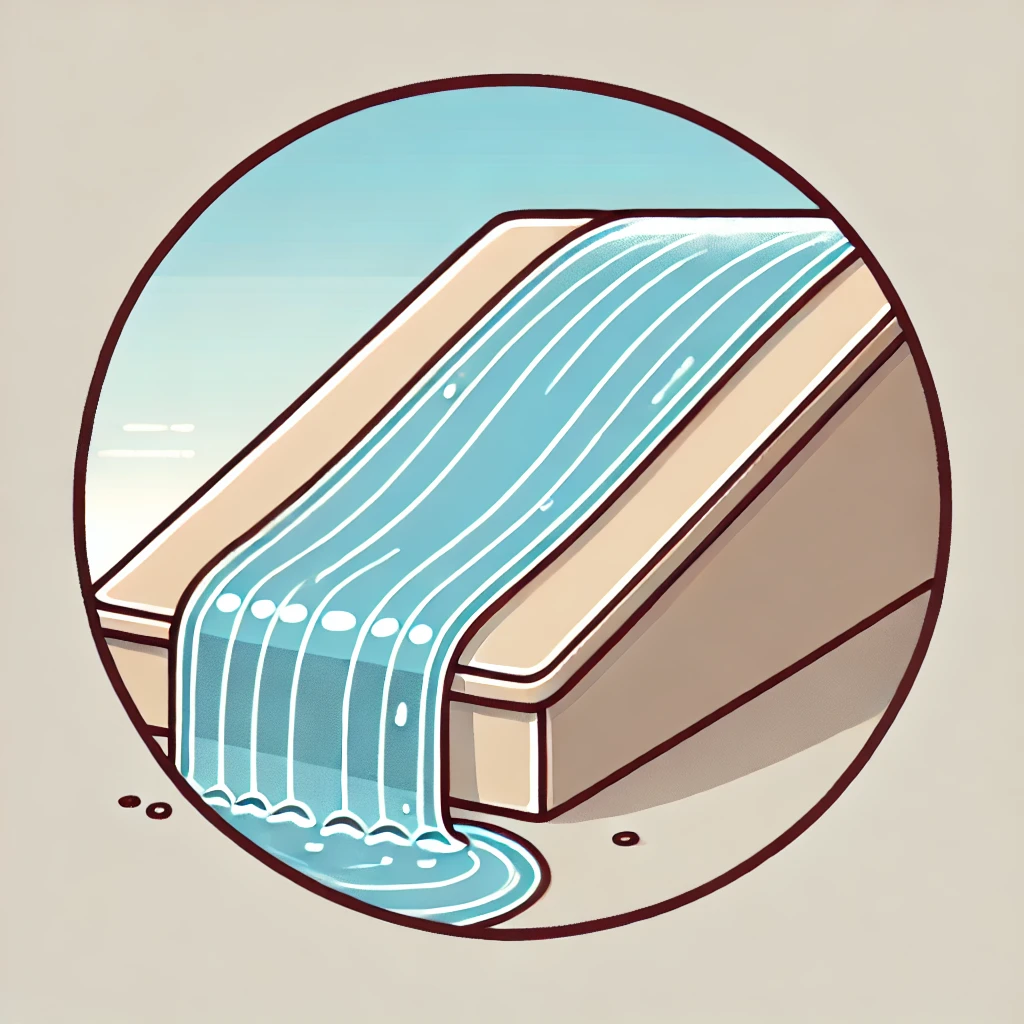
\includegraphics[width=0.4\textwidth]{cartoon_thin_film.png}
            
        \Large
        Warwick Mathematics Institute\\
        University of Warwick\\
        United Kingdom\\
        Date to fill in
    \end{center}
\end{titlepage}

\newpage

{\large \textbf{Abstract}} \\
{\normalsize The purpose of this report is to detail what I worked on during my visit at the University of Warwick with Dr. Susana Gomes and Dr. Radu Cimpeanu in the Mathematical Institute of Warwick. First of all, I simulated numerically a reduced order model of the Navier-stokes equations called the Kuramoto Shivashinski equation. Observing its numerical behaviour allowed me to familiarize with a simple reduced order model for thin film fluids. Then, I leant on the problem of stabilizing a falling liquid film with blowing air jets control, which is the main study of my report. To do so, I adapted another reduced order model, called the Benney equation, to air jet perturbation. Then, we constructed a control from the Benney equation of the system that stabilizes the system as wanted.} \\
\vspace{0.8cm} \\
{\large \textbf{Keywords}: \normalsize Feedback control, Stabilization, Thin liquid films, Air jets control, Asymptotic analysis, Reduced order modelling, LQR control, positive control.}


\newpage
\tableofcontents
\newpage



%%%%%%%%%%%%%%%%%%%%%%%%%%%%%%%%%
\section{Introduction}
Thin film fluids flows are flows which thickness are small compared to their length, this approximation being known as
 thin film approximation. We study in this report the stabilization of a thin fluid falling down an inclined plane of 
 slope angle $\theta$. Our goal is to make  a wavy thin film fluid flat by the use of controlled perturbation 
 induced by air jets. Thin film systems can typically be found in coating processes (e.g for LCD screens), heat transfer,
  and many more applications.\\

The literature covering thin film system is significantly large. Indeed, these systems provide a way to bypass the complexity 
of the Navier-Stokes equations by simplifying them with asymptotic theory, using the thin film approximation. Consequently, 
one can perform deeper mathematical studies and less computationally heavy numerical experiments. Three types of reduced order 
models, here listed with increasing complexity, are often studied: the KS (Kuramoto Shivashinski) equation, the Benney equation,
 and the Weighted Residuals. Naturally, simpler equations allows deeper mathematical and numerical studies of the equations. As 
 for the control of these flows, there is a rich literature on fluid blowing and suction based control, i.e injecting or sucking 
 fluid from the base of the plane. In her thesis, Dr.Susana Gomes built a control that could stabilize the KS system to any 
 wanted state (\cite{Susana_thesis}). However, the controls derived from this equations aren't efficient for the Benney and 
 Weighted Residual systems as the structure of the equation are probably too different. In \cite{Thompson_2016_prop_ctrl}, A.Thompson 
 and al. studied proportional control and LQR control for the Benney and Weighted Residual Systems. They studied both the continuous 
 case and discrete case, i.e with a continuum or finite number of actuators. They carried out stability analysis on the Benney and
  Weighted Residual systems and found that they could stabilize both systems with finite numbers of actuators and observations. 
  Finally, O.Holroyd and al. used in \cite{holroyd2023linearquadraticregulationcontrol} LQR control on Benney and Weighted Residual 
  systems with full observations coupled with Direct Numerical Simulation (DNS) update to link the reduced order models to more 
  realistic simulations, which they call "numerical experiments". They found that the control works successfully beyond the linear
   theory stability range. Further in \cite{holroyd2024stabilisationfallingliquidfilms}, they tackled the problem of partial observability,
    and likewise, built control scheme that would stabilize the system, although in a smaller domain of Reynolds numbers. All in all, the
blowing and suction method of actuation is thus backed with solid results. Further improvement on this control method would probably 
be to test it on a 3D system, remove the periodicity along the plane axis, and test it in a real experimental setting. These improvement 
are obviously non easy to do and would need much work like in \cite{Experimental_DNS_Reduced_order_modelling_paper} where Fabian.D and al. 
constructed an experimental setup and made comparison between experimental results, DNS results and reduced order model results. 
\\

However, blowing and sucking fluid from the base of the plane doesn't seem practical in an industrial context. One would need to drill several holes into the plane and create efficient fluid blowing and sucking pipes. Hence, we are interested in another way of introducing perturbation to the system: \underline{blowing air through pipes above the plane}. This method seem to be more practical in an industrial framework as blowing air jet seems to be far more used and easy to construct and use than liquid blowing and sucking pipes. It introduces two main difficulties. Firstly, the control has to be positive as we want blowing air jets only. Secondly, we would need to solve Navier-Stokes in the gas domain to have the link between the power of the air jet and its effect on the liquid-gaz interface which is namely the normal and tangential pressure it induces on the liquid. In \cite{Dewetting_Ojiako}, Chinasaka.J and al. showed with deep numerical analysis that the tangential part of the pressure has a non negligible effect (same amplitude as 10\% of the normal stress) on the liquid-gaz interface flat water trapped in a beacon. However, this is probably due to the fact that the water is immobile, trapped, and the air jet are strong enough to induce large deformation, until dewetting which is not the case in our system.  
In \cite{Moving_pressure_source}, D.Lunz and al. studied the effects of an oscillating actuators on a falling liquid film and carried out a analysis depending on the oscillation frequency. They simplified the problem by only modelling the normal stress induced by the gas on the liquid.  In this report, we also chose to simplify the system and only consider normal pressure, and we justify this choice later. To the best of the author's knowledge, no control paper has been drawn up with this specific system and way of control. 
\\

The report is structured in two main parts. First, we model and observe in \eqref{Section_KS_eq} the KS equation 
as an introductory work. We solve the equation numerically using an Implicit-Explicit method provided in 
\cite{Scheme_for_KS} and observe the main behaviours (steady states, progressive waves) of the KS equation, except its chaotic 
behaviour. Secondly, we study the inclined plane system: in \eqref{Section_Benney_eq}, we derive the Benney equation with a 
normal gaz pressure control term. We introduce the normal and tangential terms of the gas stress, neglect the tangential 
term, and choose a classic scaling to make the normal term appear in the equation.  Then, in \eqref{Section_Numerical_simu}, 
we construct numerical simulation scheme and carry out tests to ensure its accuracy. Finally, in \eqref{Section_Control}, we 
use the linearised Benney equation to compute a linear controls. We find that LQR state feedback control works well and stabilizes
 exponentially quickly the system. As that method gives control of any sign, we need to restraint the control to positive values to 
 have blowing only air jets. We find that LQR optimal control with just the positive part of the control applied at each time step stabilizes 
 successfully the system too, although with less efficiency. However, using this method, we are not sure that the state (i.e the height the the 
 liquid film) of the system will stay positive. Hence, we lean on another way of linear feedback control, using theory of positive control systems. 
\\

Throughout all that document, I denote: 
\begin{itemize}
    \item dimensional quantities with a * (e.g $x^*$), 
    \item non-dimensional one without anything (e.g x), 
    \item derivation with a "," e.g. $f_{,xy} = \frac{\partial^2 f}{\partial x\partial y}.$
\end{itemize}

\newpage
\section{Study of the KS equation}\label{Section_KS_eq}


In this section of the report, we study the Kuramoto Shivashinki (KS) equation which is known to be one of the simplest equations having an chaotic behaviour.  The goal of this part is not to get new results or make deep analysis as it is more an introductory part of my visit. Here, we will use specific numerical scheme and change parameters to observe the various behaviours of the numerical solutions of this equation. 

\subsection{The system and the KS equation}

The KS or Kuramoto-Shivashinski equation was first introduced by G.Shivashinsky and D.M.Michelson in 1977 in \cite{Shiv_Michelson_KS_eq} to describe flame fronts, and in 1978 by Y.Kuramoto in \cite{Kuramoto_KS_eq} to study chaotic behaviors in chemical reactions. Several other type of KS equation exists, e.g stochastic KS equation that adds  a linear stochastic term. For more details, see the thesis of Dr.Susana Gomes \cite{Susana_thesis}. One of its version is

\begin{equation}\label{KS_eq_L}
\left\{
\begin{aligned}
    u_{,t} + u_{,xxxx}  + u_{,xx} + uu_{,x} = 0 \\
    u(x+L)=u(x). 
\end{aligned}
\right.
\end{equation}



Here, we use this equation to model Falling Liquid Flow down an inclined plane in a 2D setting. The plane has a finite length L along its axis, the x-axis, which constitutes the flowing direction of the liquid. We consider the liquid being L-periodic. 
The KS equation can be derived from the Benney equation, which is a reduced order equation obtained from the 2D Navier Stokes equations. The Benney equation is presented latter in part \ref{Section_Benney_eq}. We put the derivation of the KS equation in appendix. 

Here, nor the slope angle $\theta$ or other parameters like Reynolds or Capillary numbers appear due to the way the KS equation is derived as the change of variable (not possible for all value of Reynolds number and theta) make all the variables disappear and the only variable which can be changed is the nondimensionnal length L of the domain. 
\\

\textbf{Description of the terms}
One of the benefits of the KS equation is that it is a weakly non linear equation which means that its non-linearities aren't too complex compared to other long wave models like the Benney equation or the Weighted Residuals. This weak nonlinearity $uu_{,x}$ allows in one hand deep mathematical studies, as said in introduction, but also chaotic behaviors (non linear part). This non linearity is called "Burger non linearity" referring to the Burgers equation:

\begin{equation*}
    \left\{
    \begin{aligned}
        y_{,t}(x, t) + yy_{,x}(x, t) = 0, \quad  (x,t) \in \mathbb{R}\times \mathbb{R}_+\\
        y(., t=0)=y_0(.)
    \end{aligned}
    \right.
\end{equation*}

were the only non linearity is the same as the one in the KS equation.

\textbf{Rescaling}
Let introduce what we call the instability parameter \begin{equation}
    \nu = \left( \frac{2\pi}{L}\right)^2.
\end{equation}
We make the change of variable:
\begin{equation}
    \tilde{x}= \frac{2\pi}{L}x = \frac{x}{\sqrt{\nu}},\quad \tilde{t}=\left( \frac{2\pi}{L}\right)^2t =\frac{t}{\nu},\quad  \tilde{u}=\frac{L}{2\pi}u=\sqrt{\nu}u.
\end{equation}

We keep the same notation and remove the " $\tilde{}$ " from the letters. We are now studying an equation on the domain $[0,2\pi)$ and not [0,L): 


\begin{equation}\label{KS_eq_2pi}
\left\{
\begin{aligned}
    u_{,t}  + \nu u_{,xxxx} + u_{,xx} + uu_{,x} = 0 \\
    u(x+2\pi)=u(x). 
\end{aligned}
\right.
\end{equation}

We see that the factor $\nu$ appeared in the equation. Its value will change the behaviour of the numerical solution, from steady states to chaos, as we will see in the simulations. That is why it is called "instability parameter".

\underline{\textbf{The system.}} We are studying this equation in the domain $[0, 2\pi)$ which is equivalent to study it on [0, L) with $L=\frac{2\pi}{\sqrt{\nu}}$. We will input periodic sinusoidal initial conditions and observe how they will behave depending on the frequency of the Initial condition and the value of $\nu$. We don't set a particular final time T as it could change depending on what we want to see.
\subsection{The numerical scheme}
In this section, we use the scheme described in \cite{Scheme_for_KS}. In the cited paper, the authors use it for a more complex system of equations as they try to model the dynamics of the fluids height and a surfactant. 
Here, we don't justify that the numerical scheme is appropriate for the KS equation. One just needs to take a null surfactant concentration and look at the explanation of the cited paper (essentially need to prove the regularity of the linear and non linear operators that describes the equation).  

\subsubsection{Decomposition in Fourier series}
We rewrite the KS equation \ref{KS_eq_2pi}: 

\begin{equation}\label{KS_eq_2pi_1/nu}
\left\{
\begin{aligned}
    u_{,t}  + \nu u_{,xxxx} + u_{,xx} + \frac{1}{\nu}u=\frac{1}{\nu}u -uu_{,x}  \\
    u(x+2\pi)=u(x). 
\end{aligned}
\right.
\end{equation}

We added the $\frac{1}{\nu}u$ term because we reproduced the scheme constructed in \cite{Scheme_for_KS}. It seems that it is useful to prove that the implicit-explicit scheme of \cite{KS_scheme_C_A} can be used on the KS equation. The quantities on the left will be treated implicitly and the one on the right explicitly as we will se later.
\\

As the function u in the KS equation (\ref{KS_eq_2pi}) is $2\pi$-periodic, we decompose it into its Fourier series. As u is real, we can decompose it for sin and cos components:

\begin{equation}\label{u_Fourier_serie}
    u(x, t) = \sum_{j=1}^{+\infty} u_j^ccos(jx) + u_j^ssin(jx) + \bar{u}(t),
\end{equation}


$$u^c=(u_j^c)_{j\in \mathbb{N}^*}, u^s= (u_j^s)_{j\in\mathbb{N}^*}, \bar{u}$$ being respectively the cos, sin components and the mean value of u. 

As we studying the steady state u=0, we take centered sinusoidal initial conditions and suppose here that $$\bar{u}=0.$$


Using the Fourier series in \ref{KS_eq_2pi}, we have that

\begin{align*}
  u_{,t}  + \nu u_{,xxxx} + u_{,xx} + \frac{1}{\nu}u &= \sum_{j=1}^{\infty} (\frac{du_j^c}{dt} + (\nu j^4 - j^2)u_j^c +\frac{1}{\nu}u_j^c)cos(jx) \\ &+ \sum_{j=1}^{\infty}(\frac{du_j^s}{dt} + (\nu j^4 - j^2)u_j^s +\frac{1}{\nu}u_j^s)sin(jx)\\ &= \sum_{j=1}^{\infty} (\frac{1}{\nu}u_j^c- F_j^c)cos(jx)  +(\frac{1}{\nu}u_j^s- F_j^s)sin(jx) \\ &= \frac{1}{\nu}u - uu_{,x},
\end{align*}

with 
\begin{align*}
F_j^c = -\frac{j}{2} \sum_{m+n=j}u_m^cu_n^s + \frac{j}{2} \sum_{m-n=j}(u_m^cu_n^s - u_n^cu_m^s), \\
F_j^s = \frac{j}{4} \sum_{m+n=j}(u_m^cu_n^c - u_m^su_n^s)+ \frac{j}{2} \sum_{m-n=j}(u_m^cu_n^c + u_n^su_m^s)
\end{align*}

the Fourier cross terms induced by the weak non-linearity of the KS equation. 

By projecting the inequality on $(cos(jx)_{j\in \mathbb{N}^*}, (sin(jx)_{j \in \mathbb{N}^*})$,  Orthogonal family of vectors in $L^2([0,2\pi), \mathbb{R})$, we have an infinite number of Ordinal Differential Equations (ODEs): 

\begin{equation}\label{ODE_KS}
    \forall j \in \mathbb{N}^*,\quad 
    \left\{
    \begin{aligned}
        \frac{du_j^c}{dt} + (\lambda_j + \frac{1}{\nu})u_j^c = \frac{1}{\nu}u_j^c + F_j^c \\
        \frac{du_j^s}{dt} + (\lambda_j + \frac{1}{\nu})u_j^s = \frac{1}{\nu}u_j^c + F_j^s
    \end{aligned}
    \right.
\end{equation}

with 
\begin{equation}
    \forall j\in \mathbb{N}^*, \quad \lambda_j = \nu j^4 - j^2 = \nu j^2(j-\frac{1}{\sqrt{\nu}})(j+\frac{1}{\sqrt{\nu}}).
\end{equation}

 First of all, we don't simplify the $u_j^c$, $u_j^s$ in the equation as one will be implicit and the other explicit in the numerical scheme that we will describe in an instant. 

Let us underline that the equations in (\ref{ODE_KS}) have exponential solutions of rate $\lambda_j$ when there is no weak non linearity terms $F_j^{c,s}$ i.e equations of the form \begin{equation}\label{KS_exponential_ODE}
    \forall j\in \mathbb{N}, \quad \frac{du_j^{c,s}}{dt} = -\lambda_ju_j^{c,s}.
\end{equation}

\underline{\textbf{Sign of the } $\boldsymbol{\lambda_j}.$} If we neglect the non-linearities, we remark that we would have an exponential dampening on the $j^{th}$ mode if and only if $$-\lambda_j > 0. $$

When $\forall j \in \mathbb{N}^*,\lambda_j <0,$ we are expecting the non-linearities will be indeed negligible if we take a low number of initial mode as the the $F_j^{c,s}$ will be small at the beginning so the derivatives of the $u_j^{c,s}$ will still be negative. 
At the opposite, if $\exists j \in \mathbb{N}, \quad \lambda_j >0$ then if we take the non-linearities small enough at the beginning,$u_j$ will grow and its effect will spread in the other $u_i$ through the non-linearities $F_j^c$ and $F_j^s$. Therefore, we will try later to control the signs of the $\lambda_j$.



\subsection{Description of the scheme}

Here, we first present the equations (\ref{ODE_KS}) in a specific way, discretize it for it to be suitable for numerical program, and then introduce the numerical scheme that we are going to use. 
\\

we set 
\begin{equation}
    U = (u^c, u^s) \in \mathbb{R}^{\mathbb{N}^*} \times\mathbb{R}^{\mathbb{N}^*}
\end{equation} the grouping of the 2 vectors of the Fourier coefficients of u .

Equations (\ref{ODE_KS}) can be rewritten as 

\begin{equation}
    \frac{dU}{dt} + A(U) = B(U)
\end{equation}
with 

$$AU = \left((\lambda_j + \frac{1}{\nu})u^c_j, (\lambda_j + \frac{1}{\nu})u^c_j\right)_{j \in \mathbb{N}}, \quad B(U) = \left(\frac{1}{\nu}u_j^c + F_j^c, \frac{1}{\nu}u_j^s + F_j^s\right)_{j\in \mathbb{N}}$$
so A and B are respectively a linear and non-linear operators.
\\

\textbf{The numerical Scheme.} We describe now the numerical scheme used by \cite{Scheme_for_KS}. They used a Implicit-Explicit multi-step method introduced and analyzed in \cite{KS_scheme_C_A} by G.Akrivis and M.Crouzeix. We will see it is an implicit BDF (Backward Differentiation Formula) scheme of order 
\begin{equation}
    p_{BDF} \in \mathbb{N}^*
\end{equation} for the time derivative and the linearity, combined with a multi-step explicit scheme for the non-linearity. 
\\

Let us now set $N_x, N_t$ the number of space and time points respectively. Then $$dt = \frac{T}{N_t-1},\quad dx = \frac{2\pi}{N_x}.$$ 

Let us then set $$\forall n\in [|0, N_t-1|], \quad U^n = U(ndt) = ((u_j^c(ndt)_{j\in \mathbb{N}}, (u_j^s(ndt))_{j\in \mathbb{N}}).$$

We introduce the polynomials of degree $p_{BDF}$
 \begin{equation}
     \alpha = \sum_{i=1}^{p_{BDF}} \frac{1}{j}X^{p_{BDF}-1}(X-1)^j, \quad  \beta = X^{p_{BDF}}, \quad \gamma = X^p_{BDF} - (X-1)^{p_{BDF}} \in \mathbb{R}_{p_{BDF}}[X].
 \end{equation}

The numerical scheme for the time is constructed with $(\alpha, \beta)$ with implicit scheme and the non linearity is managed with $(\alpha, \gamma)$. Both schemes are of order $p_{BDF}$:

\begin{equation}
    \sum_{i=0}^p \alpha_i U^{n+i} + dt\beta_{p_{BDF}}AU^{n+p} = dt\sum_{i=0}^{p-1} \gamma_iB(U^{n+i}), \quad n\in [|0, N-p|]
\end{equation}

with $\alpha_i, \beta_i, \gamma_i$ being the coefficients of order i of $\alpha, \beta,$ and $\gamma$ respectively. The scheme is therefore: 
\\

\begin{equation}
    \boxed{
    \sum_{i=0}^p \alpha_i U^{n+i} + dtAU^{n+p} = dt\sum_{i=0}^{p-1} \gamma_iB(U^{n+i}), \quad n\in [|0, N-p|]
    }
\end{equation}

We then truncate U up to a certain order to do numerical computations. We get $$U^{d, n} = \left((u_j^c(ndt))_{j\in [|1,d|]}, (u_j^s(ndt))_{j\in [|1,d|]} \right)\in \mathbb{R}^{2d},$$ 
$A^d$ and $B^d$ the new operators defined naturally from A and B with the new truncated non linear coefficients:

\begin{equation}
\left\{
\begin{aligned}
    F_j^{d,c} &= -\frac{j}{2} \sum_{\substack{m+n=j \\ 0\leq m, n \leq d}}u_m^cu_n^s + \frac{j}{2} \sum_{\substack{m-n=j\\ 0\leq m, n \leq d}}(u_m^cu_n^s - u_n^cu_m^s) \\
    F_j^s &= \frac{j}{4} \sum_{\substack{m+n=j \\ 0\leq m, n \leq d}}(u_m^cu_n^c - u_m^su_n^s)+ \frac{j}{2} \sum_{\substack{m-n=j \\ 0\leq m, n \leq d}}(u_m^cu_n^c + u_n^su_m^s)    
\end{aligned}
\right.
\end{equation}


As we use the FFT algorithm (Fast Fourier Transform), the highest mode left is $d =\lfloor N_t/2 \rfloor.$ For more precision on the code, see the appendix \ref{KS_computation_numerics} on how we implemented it, or see also the code on the \href{https://github.com/Bilal59170/Repo_Warwick_internship}{Github page}. 

\subsection{Simulations and Results}
We implement all the simulations in a python file. They can be found in \href{https://github.com/Bilal59170/Repo_Warwick_internship}{this Github repository}.

\subsubsection{Dispersion relation}
We recall the expression of the $\lambda_j:$

\begin{equation}
    -\lambda_j = -\nu j^2(j-\frac{1}{\sqrt{\nu}})(j+\frac{1}{\sqrt{\nu}})
\end{equation}

As we said earlier, we want to know the sign of the $\lambda_j$. We know it just by analyzing the polynomials of order 4 in j. We have that

\begin{equation}
\left\{
\begin{aligned}
    -\lambda(j) > 0 \quad  \text{on } (0, \frac{1}{\nu}) \quad \text{(exp. growth)},\\
    -\lambda(j) < 0 \quad  \text{on } (\frac{1}{\nu}, +\infty)  \quad \text{(exp. decay)},\\
    -\lambda(j) = 0 \quad \text{on } \{0, \frac{1}{\sqrt{\nu}}\}
\end{aligned}
\right.
\end{equation}

which means that for $\nu < 1$, having j such that $-\lambda_j > 0$ is impossible. As we study a periodic function, it is a superposition of natural integer modes (cf the Fourier series of u in \ref{u_Fourier_serie}). Hence, any periodical input would be exponentially dampened in a system if there wasn't any the non-linearities. 

We show on figure \ref{fig:KS_eq_lambda_growing_and_dampening} two profiles of $\lambda_j$ for different values of $\nu$, with and without divergent modes.
\\

\begin{figure}[h]
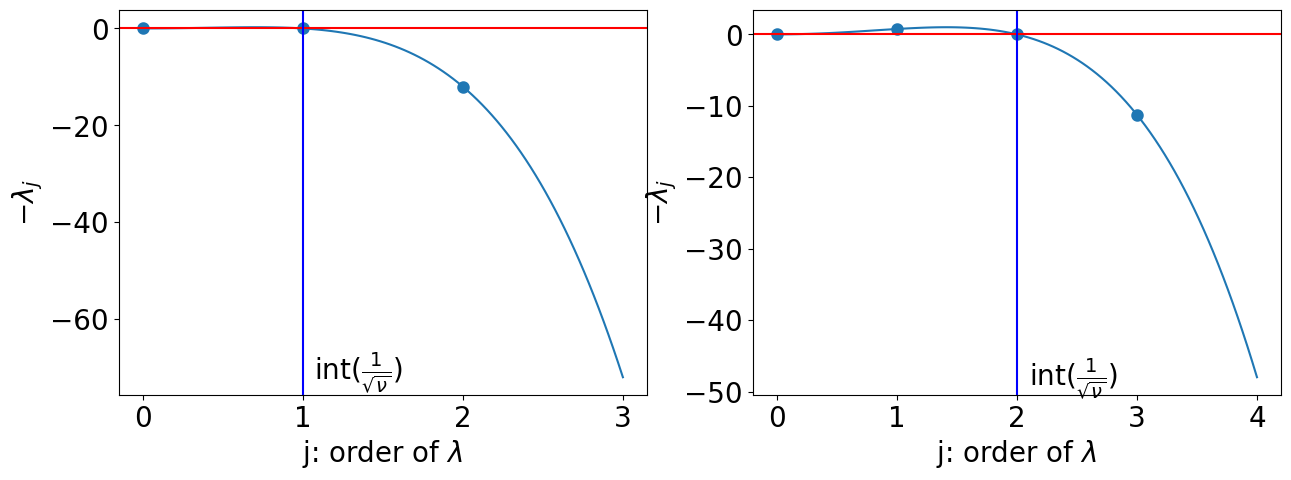
\includegraphics[width=1\textwidth]{KS_eq/plot_dispersion_nu_1_1-4.png}
\caption{Two curves of -$\lambda(j)$ for $\nu=1$ and $\nu=\frac{1}{4}$. The first case gives no exponentially growing regime, but the second case does with $\lambda_1 >0$. } 
\label{fig:KS_eq_lambda_growing_and_dampening}
\end{figure}

We will now separate our observations in two parts: $\nu \geq1$ and $\nu <1$.

\subsubsection{\texorpdfstring{$\nu \geq 1$}{nu >= 1}}

As said before, we are expecting to have exponential decays. We will here measure the characteristic decay of curves as if they were decaying exponentially by computing an exponential regression (linear regression on a log scale). Then, we compare the coefficients to the expected rate. 

We carry out these tests for $\nu =1$. We compared the dampening values for $k \in {0, 1, 2, 3, 4, 5}.$We use initial condition sin(kx) and cos(kx). Except k=0, we found that for both initial conditions, the exponential regime and the curve of $u_{max}$ were identical until a floor value (around $10^{-16}$) where the solution would become flat, maybe because of the float precisions in the operations.

We are expecting of having $$log(u_{max}) = log(u_{max}(0)e^{-\lambda_k t}) = log(u_{max}(0)) -  \lambda_k t$$ with $u_{max}(t) = \max_{x\in[0,2\pi]}|u(.,t)|.$ Hence we compare the coefficient a and b from the linear regression y = ax+b to $-\lambda_k$ and $log(u_{max}(0))$ respectively with these relative errors terms: $$\eta_a = \frac{|a-(-\lambda_k)|}{|-\lambda_k|}, \eta_b = \frac{|b-log(u_{max}(0)|}{|log(u_{max(0)})|}.$$  The determination coefficient $r^2$ of the linear regression was always very high (at least 0.9999 and 1 is a perfect matching) so we don't display it. 

\begin{center}
\begin{tabular}{ |c|c|c| } 
 \hline
    Modes j  & $\eta_a$ (in \%) & $\eta_b$ (in \%)  \\
 \hline
 2 & (0.04, 0.2) & (0.4, 2) \\ 
 3 & $(2.10^{-4}, 2.10^{-3})$ & (0.01, 0.05) \\ 
 4 & $(1.10^{-6}, 1.10^{-5})$ & (0.01, 0.01) \\ 
 \hline
\end{tabular}
\end{center}

We see that we have very low error so the non-linearities in that case are quite negligible. We see that the errors are a bit higher for sin than cos initial condition, maybe because they are no crossed term (i.e $u_m^s u_n^c$ and not $u_m^c u_n^c$) in  the non linearity $F_j^s$ than in $F_j^s$. For instance, if we take sin(2x) as initial condition, non zero term will appear in $F_4^s=\frac{4}{4}(-{u_2^s}^2)$ but $F_4^c=0$. This is the case for an infinite number of modes after j=2. Therefore, the effect of the non-linearities appears the most for little modes as they make higher modes appear which creates a chain reaction . That is maybe why the relative error rate are decreasing when we test higher modes. 



\begin{figure}[htbp]
    \centering
    % First image
    \begin{minipage}[b]{0.45\textwidth}
        \centering
        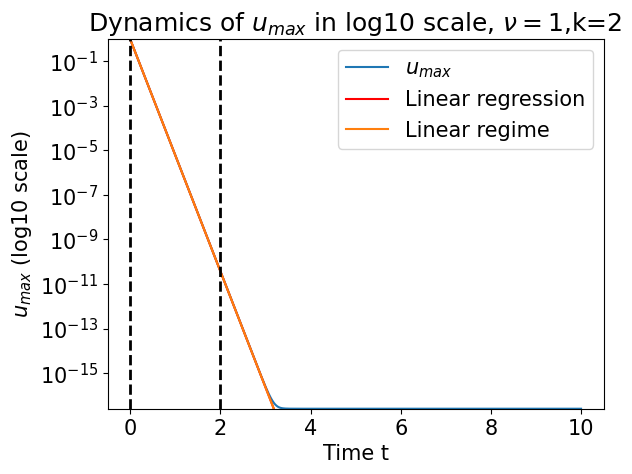
\includegraphics[width=\textwidth]{KS_eq/plot_exp_decay.png}
        \caption{Case nu=1, k=2}
        \label{fig:image1}
    \end{minipage}
    \hfill
    % Second image
    \begin{minipage}[b]{0.45\textwidth}
        \centering
        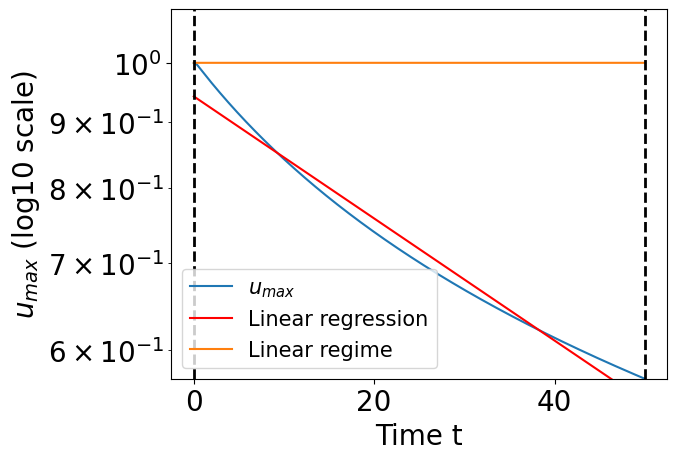
\includegraphics[width=\textwidth]{KS_eq/plot_decay_nu_1_k_1png.png}
        \caption{Case nu=1, k=1}
        \label{fig:image2}
    \end{minipage}
    \caption{Figure of the exponential decay of $log(max|u(.,t)|)$ and its comparison with the linear regime in the case where the initial condition is a mode of order 1 (right) i.e cos or sin and 2 (left). \\
    The left part behave almost exactly like the linear regime. As for the right plot, instead of staying still, the initial condition decreases in norm because of the non-linearities. The black horizontal dots are delimiting the domain where the linear regression has been made.}
    \label{fig:both_images}
\end{figure}

In opposite to the previous cases, the case j=1 is different to the linear regime which should be just stationary. In the same spirit than the remark above, we think that all the non-linearities $F_{j'}$ of the modes after $j'>j=1$ are non zero. The main mode j=1 doesn't become small quickly like the previous cases, so the non-linearities $F_{j'}$ become non negligible too and make the function non stationary. However, we don't know why they make the function decrease.

\subsubsection{\texorpdfstring{$\nu <1$}{nu < 1}}
We now look at the case we $\nu <1$. It is expected to have far more complex behaviour than when $\nu \geq 1$ as we can have here exponentially growing modes interacting with each other. We will observe that the system seems to be more unstable with $\nu = (\frac{2\pi}{L})^2$ decreasing, i.e when L increases. 
We just observe three behaviour: exponential dampening (linear regime), stabilization around a non-zero state, and progressive wave.
\\

In opposition to the tests above, we are fixing a mode value (j=1 e.g) and change the value of $\nu$. Here is a graph of $\lambda_1(\nu)$ depending on nu < 1: 

\begin{figure}[h]
\centering
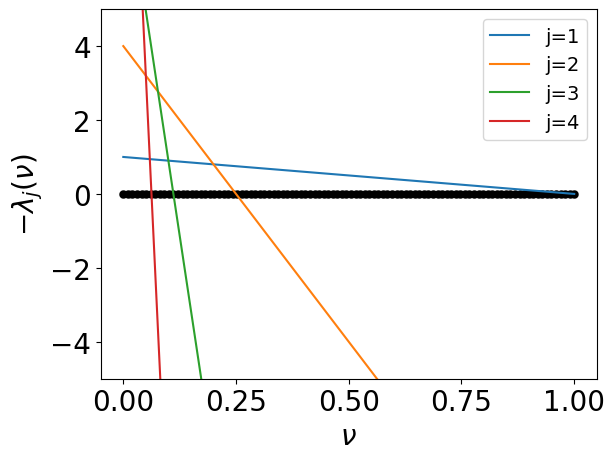
\includegraphics[width=0.5\textwidth]{KS_eq/plot_lambda_nu.png}
\caption{Plot of $-\lambda_j(\nu)$ for j $\in$ \{1, 2, 3, 4\}. We see that there are more and more positive modes when $\nu$ is decreasing. Further more, the equation is more sensitive when$\nu$  is small compared to $\nu$ near 1 as the same perturbation $\delta \nu$ around small $\nu$ could give several additional pseudo exponential growing modes.   }
\label{fig:KS_eq_nu_inf_1}
\end{figure}


\begin{figure}[h]
\centering
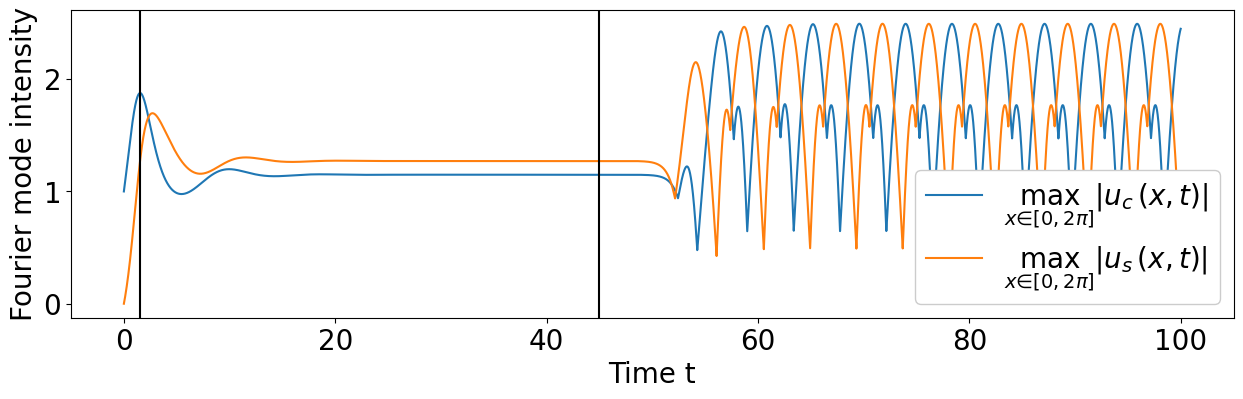
\includegraphics[width=1\textwidth]{KS_eq/KS_extrema_Fourier_coef.png}
\caption{\textbf{Case of progressive wave with }$\boldsymbol{\nu=7/24}$: \\ We see here 3 behaviours. Growing, decreasing and stabilization around a non flat state, and than a progressive wave behaviour. Indeed, we can see that the extrema if the cos and sin modes are oscillating at a fixed frequency which shows the progressive characteristic of the wave (we also saw it in video).}
\label{fig:KS_eq_nu_inf_1}
\end{figure}


We see in \eqref{fig:KS_eq_nu_inf_1} that the case $\nu=\frac{1}{4}$ is interesting as we would have a second divergent mode. We make tests with $\nu$ getting closer to 1/4 by above ($\{\frac{1}{2}, \frac{1}{3}, \frac{7}{24} = \frac{1/3+1/4}{2}, \frac{13}{48} = \frac{7/24 + 1/4}{2}\}$). We observe two behaviours:
\begin{itemize}
    \item When $\nu$ is "far" from $\frac{1}{4}$: u grows exponentially and then stabilizes around a wavy steady state.
    \item When $\nu$ is "close" to $\frac{1}{4}$: There is also a linear regime and a stabilization around a steady. However the equilibrium breaks and it becomes a traveling wave (cf 
\end{itemize}


We don't go further for this little study of the KS equation. We analyzed the KS equation through the Fourier decomposition of u. We tried to interpret the numerical results by seeing the equation on each mode as being almost exponential. The case $\nu \geq1$ seemed to give simple result of exponential decay, while the case $\nu <1$ was more difficult to justify as modes are influencing each other in a non negligible way. 

We didn't test the other case when $\nu <\frac{1}{4}$. The KS equation seems to be more unstable as $\nu$ decreases, i.e when L increase. Hence, the domain $\nu \in (0,\frac{1}{4}] $ should be even more rich in term of behaviour as we add other exponentially growing modes.

As the KS equation is weakly linear, many mathematical studies have been carried out to study its chaotic behaviour (that we don't see here), like the study of bifurcation. We again refer to the thesis of Dr.Gomes (\cite{Susana_thesis}) for a real study of this equation.




\newpage




\section{The Benney equation with air jets actuators}\label{Section_Benney_eq}



\subsection{Derivation of the Benney Equations with and without control}
\subsubsection{Benney equation without control}

We are studying a liquid flowing down an inclined plane of angle $\theta$ in 1D from the horizontal. The system of axis $(x^*, y^*$) is such that $x^*$ points downstream and $y^*$ is normal to the plane going upward. 
\\

\vspace{0.5cm}
{\textbf{Set of dimensionnalised equations.}}
We study\\ 

The Navier-Stokes equations (2nd law of Newton and incompressibility equation):

\begin{equation}
\left\{
\begin{aligned}
    \rho(u^*_{,t^*}+u^*u^*_{,x^*}+v^*u^*_{,y^*}) &= -p^*_{,x^*} + \mu_l(u^*_{,x^*x^*} + u^*_{,y^*y^*}) + \rho sin(\theta)g\\
    \rho(v^*_{,t^*}+u^*v^*_{,x^*}+v^*v^*_{,y^*}) &= -p^*_{,y^*} + \mu_l(v^*_{,x^*x^*} + v^*_{,y^*y^*}) - \rho cos(\theta)g\\\
    u^*_{,x^*} + v^*_{,y^*} &= 0 \quad 
\end{aligned}
\right.
\end{equation}

We take a no slip boundary conditions at the wall so at y = 0\footnote{in the case of a control with blowing and suction from the plane, $v^*\neq 0$ }: 

\begin{equation}
    u^*=0, v^*=0
\end{equation} 

The normal and tangential Dynamic Boundary Condition or the dynamic stress balance at the interface are : 

\begin{equation}
\left\{
\begin{aligned}
-p^*_l + \frac{2\mu_l}{1+{h^*_{,x^*}}^2}(u^*_{,x^*}{h^*_{,x^*}}^2 - h^*_{,x^*}(u^*_{,y^*} + v^*_{,x^*})+v^*_{,y^*}) &= \frac{\gamma h^*_{,x^*x^*}}{(1+{h^*_{,x^*}}^2)^{3/2}}\\
(v^*_{,x^*} + u^*_{,y^*})(1-{h^*_{,x^*}}^2)+2h^*_{,x^*}(v^*_{,y^*}-u^*_{,x^*})&=0
\end{aligned}
\right.
\end{equation}
\\

The Kinematic Boundary condition is: 
\begin{equation}
h^*_{,t^*} = v^*-u^*h^*_{,x^*}.
\end{equation}


\vspace{0.5cm}
\textbf{Nondimensionalisation and scaling}


We now make a change of variable in order to manipulate dimensionless quantities. We denote 
\begin{itemize}
    \item $\mathcal{L^*}$ characteristic horizontal length
    \item $\mathcal{H^*}= h_N^* $ typical fluid height (and typical vertical length) which is also the \textit{Nusselt solution} i.e film height at steady state that we fix as we want.
    \item $\mathcal{U^*} := U^*_N=\frac{\rho g{h_N^*}^2 sin(\theta)}{2\mu_l}$ typical horizontal velocity and also velocity of the Nusselt solution. 
    \item $\mathcal{P^*}$ typical pressure of the liquid \\
\end{itemize}


Moreover, we make the \textbf{Thin-Film Approximation} which is to take $\mathcal{H^*} \ll \mathcal{L^*}$ i.e the width of the film is small compared to its length. We now scale the variables of the problem with the \textbf{thin-film parameter} 
\begin{equation}
\boxed{
\epsilon = \frac{\mathcal{H^*}}{\mathcal{L^*}}.
}
\end{equation}

Therefore, we get these non-dimensional quantities:: 
\begin{align*}
    x^* &= \mathcal{L^*}x, \quad y^*= \epsilon \mathcal{L^*}y, \\
    u^* &= \mathcal{U^*}u,  \quad v^*= \epsilon \mathcal{U^*}v, \\
    p_l^* &= \mathcal{P^*}p_l
\end{align*}

where we took the typical vertical velocity equal to $\mathcal{V}^*:=\epsilon\mathcal{U}^*.$ We now take some convenient form for the typical pressure: $\mathcal{P^*} = \frac{\mu_lU^*}{h_N^*}$ and set the nondimensionalised quantities (Reynolds and Capillary numbers): 

\begin{equation}
    \boxed{
    Re = \frac{\rho \mathcal{U^*} h_N}{\mu_l} \quad Ca = \frac{\mu_l \mathcal{U^*}}{\gamma}.
    }
\end{equation}
\\

We choose the scaling 
\begin{equation}
Re=O(1) \text{ and } Ca=O(\epsilon^2). 
\end{equation}

The first scaling allow to consider inertia whereas the second one underlines surface effect in the order 1 approximation in $\epsilon$ that we will carry out. 
Indeed, the effect of interest here are \textbf{viscosity}, \textbf{surface tension}, \textbf{gravity} and \textbf{inertia}. These 4 effects are balanced by the 3 quantities Re, Ca and $U_N$ the Nusselt velocity which is a function of the slope angle $\theta$.
\\
            
 \textbf{Non-dimensional governing equations.} We present the new equation with dimensionless variable.

First, we have the Navier-Stokes equation:
\begin{equation}\label{eq NavierStokes1}
\left\{
\begin{aligned}
    Re(u_{,t}+uu_{,x}+vu_{,y}) &= -p_{,x} + u_{,xx} + u_{,yy} + 2\\
    Re(u_{,t}+uu_{,x}+vu_{,y}) &= -p_{,x} + u_{,xx} + u_{,yy} + 2 + v_{,yy} - \rho cos(\theta)g\\
     u_{,x} + v_{,y} &= 0 
\end{aligned}
\right.
\end{equation}


Then, the no slip condition: 
\begin{equation}\label{eq_no_slip}
    u=0, \quad v=0 \quad \text{at y=0,}
\end{equation}

the Dynamic stress balance at the interface: 

 

\begin{equation}\label{eq DBC}
\left\{
\begin{aligned}
    - p_l + \frac{2}{1+{h_{,x}}^2}(u_{,x}{h_{,x}}^2 - h_{,x}(u_{,y} + v_{,x})+v_{,y}) &= \frac{1}{Ca} \frac{h_{,xx}}{(1+{h_{,x}}^2)^{3/2}}\\
    (v_{,x} + u_{,y})(1-{h_{,x}}^2)+2h_{,x}(v_{,y}-u_{,x})&=0
\end{aligned}
\right.,
\end{equation}


and finally, the Kinematic Boundary condition (KBC): 
\begin{equation}\label{eq KBC}
    h_{,t} = v-uh_{,x}.
\end{equation}

From \ref{eq KBC} and \ref{eq NavierStokes1} and  \ref{eq_no_slip}, i.e the KBC, incompressibility, and no slip equations, we can construct the 1D mass conservation equation: 
\begin{equation}\label{eq mass conservation}
    h_{,t} + q_{,x} = 0
\end{equation}

with $$q(x, t) = \int_{y=0}^{h_(x, t)} u(x, y, t)dy$$ the horizontal flux of the flowing liquid.

\vspace{0.5cm}
{\textbf{Benney equation}}

With the chosen scaling, we perform order 1 asymptotics in $\epsilon$ on the governing equations and compute the order 1 flux. These computations can be found in \cite{A_Thompson_FLF_blowing_suction}. It leads us to the so called Benney equations: 

\begin{equation}
    \boxed{
\begin{aligned}
    h_{,t}+q_{,x} &= 0\\
    q(x, t) &= \frac{h^3}{3}(2-2h_{,x}cot(\theta) + \frac{h_{,xxx}}{Ca})+Re\frac{8h^6h_{,x}}{15}.
\end{aligned}
}
\end{equation}

i.e

\begin{equation}\label{Benney_eq}
\boxed{
\begin{aligned}
    h_{,t} &+ h_{,x}h^2 \left( 2-2h_{,x}cot(\theta) + \frac{h_{,xxx}}{Ca}\right) \\ &- \frac{h^3}{3}\left( 2h_{,xx}cot(\theta) - \frac{h_{,xxxx}}{Ca} \right) + \frac{8Re}{15} \left( 6h^5 {h_{,x}}^2 + h^6 h_{,xx} \right) = 0.
\end{aligned}    
}
\end{equation}




\subsubsection{Benney equation with a control term}
We want to stabilize the fluid by applying some air jet controlled perturbation. However, we do not model the air and just take a specific form of the normal pressure (e.g. gaussian). Let us write 

\begin{equation}
    \underline{s_g}= -\underline{n}.\underline{\underline{\sigma_l}}
\end{equation}
with $\underline{\underline{\sigma_l}}$ the tensor of constraint of the liquid, and $\underline{n}$ the normal \underline{from the liquid to the gas} We take as normal and tangential vectors $(\underline{n}, \underline{t})$ a normalized, orthogonal and direct couple. We then isolate the normal and tangential components of the external gas pressure. 

 \begin{equation}
     \underline{n}=\frac{1}{\sqrt{1+h_{,x}^2}}(-h_{,x}, 1), \quad \underline{t} = \sqrt{1+h_{,x}^2}(1, h_{,x}),
 \end{equation}

\begin{equation}
    \boxed{
    (N_s, T_s) =  \underline{s_g}(y=h).\underline{n}.
    }
\end{equation}

Let us emphasize that we took the sign convention of $N_s$ such that it is positive with a compressive force, as $\underline{s_g}$ is defined with a -\underline{n} which points \underline{from the gas to the liquid}. 

As for the governing equations, only the KBC changes: 

\begin{equation}\label{eq DBC_Control}
    \left\{
    \begin{aligned}
    -p_l + \frac{2}{1+{h_{,x}}^2}(u_{,x}{h_{,x}}^2 - h_{,x}(u_{,y} + v_{,x})+v_{,y}) &= \frac{1}{Ca} \frac{h_{,xx}}{(1+{h_{,x}}^2)^{3/2}}-N_s \\
    \frac{(v_{,x} + u_{,y})(1-{h_{,x}}^2)+2h_{,x}(v_{,y}-u_{,x})}{1+h_{,x}^2} &= -T_s.
    \end{aligned}
    \right.
\end{equation}

Howewer, only the normal KBC changes in reality as we take  
\begin{equation}
T_s=0
\end{equation} 
which means that we neglect the tangential part of the stress of the gas on the liquid.  This approximation has been made by the paper 
of D.Lunz \& al. \cite{Moving_pressure_source} but it has been shown on another system studied by Chinasa J. Ojiako \& al. in
 (\cite{Dewetting_Ojiako}) that the tangential component of the air jet pressure has non negligible effects on the profile of the liquid. 
 We decide not to take into account the tangential stress for two reasons.
\begin{itemize}
    \item Firstly, we think that the tangential part of the air stress on the liquid was important (around 10\% of the normal
     stress $N_s$) in the case of the paper of Chinasa J. Ojiako because the air was blown on immobile flat water, so the trough 
     produced by the air jet would prevent air from escaping by the sides. This effect is probably largely attenuated in our system 
     since the fluids are here driven by gravity and inertia, so there are much fluid movement that would allow the gas to come out 
     easily by the sides. 
    \item Secondly, considering $T_s$ would add too much complexity to our model. We prefer to construct a simple model on which
     we can apply a control strategy more easily, as we will see after. Another work on constructing an equation and control strategy while taking into account $T_s$ could be made and compared to this one.
\end{itemize}


\textbf{Benney equation with control.}
The computation of the pressure is different (cf Appendix) and it gives at order 1 in $\epsilon$:

\begin{equation}\label{Benney_ctrl_flux}
\boxed{
\begin{aligned}
    h_{,t}+q_{,x} &= 0\\
    q(x, t) &= \frac{h^3}{3}(2-p_{l0,x})+Re\frac{8h^6h_{x,}}{15}
\end{aligned}
}
\end{equation}

with 
\begin{equation}
p_{l0}= N_s + 2(h-y)cot(\theta) - \frac{h_{,xx}}{Ca},
\end{equation}
the pressure term approximated at order 0.

Hence, the Benney equation with only h as unknown is 
\begin{equation}\label{Benney_eq_ctrl}
\boxed{
\begin{aligned}
    h_{,t} &+ h_{,x}h^2 \left( 2-N_{s, x}-2h_{,x}cot(\theta) + \frac{h_{,xxx}}{Ca}\right) \\ &- \frac{h^3}{3}\left(N_{s, xx} + 2h_{,xx}cot(\theta)  - \frac{h_{,xxxx}}{Ca} \right)
    + \frac{8Re}{15} \left( 6h^5 {h_{,x}}^2 + h^6 h_{,xx} \right) = 0
\end{aligned}
}.
\end{equation}

\subsubsection{Linear Theory}\label{subsubsection_linear_theory}
In this section, we present some theory relying on the linearisation of the Benney equation. 

We write the height as a perturbed state from the Nusselt height 1 : 
\begin{equation}\label{h_linear_decomposition}
    h = 1+\delta \tilde{h},\quad N_s = \delta \tilde{N}_s
\end{equation}

Let us underline that $\delta$ and $\epsilon$ aren't linked. The $\epsilon$ parameter gives the relation between the Nusselt height and L and ensures (when very small) that the derivation of the Benney equation is valid. As for $\delta$, it is a parameter that appears after the nondimensionalisation and just ensures that the perturbation has small amplitude compared to 1, the normalized Nusselt height. 

We then keep the term of the Benney equation with control (\ref{Benney_eq_ctrl}) until order 1 in $\delta$ included. It gives a linear equation that we will use for the control:

\begin{equation}\label{Benney_ctrl_linearised}
    \tilde{h}_{,t} = \left[ -2\partial_x + (\frac{2cot(\theta)}{3}-\frac{8Re}{15})\partial_{xx} - \frac{1}{3Ca}\partial_{xxxx}\right]\tilde{h} + \left[ \frac{1}{3}\partial_{xx}\right]\tilde{N}_s
\end{equation}
\\
We study here the case $$\tilde{N}_s = 0.$$
We decompose $\tilde{h}$ as $$\tilde{h}(x,t) = \sum_{k\in\mathbb{Z}}c_k(t)e^{i\nu kx}$$

with $\nu =\frac{2\pi}{L}$ as $\tilde{h}$ is L-periodic.So (time derivation+ Fourier base identification)we have $\mathbb{Z}$ number of ODEs: 
\begin{equation}\label{Fourier_mode}
    c_{k, t}(t) = \lambda_k c_k(t)
\end{equation}
with 

\begin{equation*}
\begin{aligned}
    \forall k\in \mathbb{Z},\\
    \lambda_k &= (ik_L)^4(\frac{-1}{3Ca})+(ik_L)^2(\frac{2}{3}cot(\theta)-\frac{8Re}{15})-2k_Li \\
    &= (\frac{8Re}{15}-\frac{2}{3}cot(\theta) -\frac{k_L^2}{3Ca})k_L^2 - 2k_Li, \\ \\
    k_L &= \nu k.
\end{aligned}
\end{equation*}

Let us set \begin{equation}
    Re_0 = \frac{5}{4}cot(\theta)
\end{equation}
like in A.Thompson and al. paper \cite{Thompson_2016_prop_ctrl}.

The dispersion equation is then 
\begin{equation}\label{dispersion_relation}
\boxed{
    \lambda_k = -2ik_L+ \frac{8}{15}\left( Re-Re_0-\frac{5k_L^2}{8}\right)k_L^2
}
\end{equation}
The \textbf{stability} of the linear system is determined by a condition on the real part of the eigenvalues: $$\mathcal{R}(\lambda_k)\leq0.$$

$\mathcal{R}(\lambda_k) = P(\lambda_k^2)$ with P a polynomial of order 2 going to minus infinity at infinity. Hence, the unstable/diverging modes k verify 
\begin{equation}
|k|\leq k_0 := \sqrt{Ca(\frac{8}{5}Re-2cot(\theta)} = \sqrt{\frac{8Ca}{5}(Re-Re_0)}.
\end{equation}

We see that if $Re<Re_0$, there is no unstable modes. Having a larger Reynolds number would give more place to inertia and so more chance to have a chaotic flow. Therefore, we call $Re_0$ the unstable Reynolds number.

\newpage





\section{Numerical simulations}\label{Section_Numerical_simu}
\subsection{Description of the numerical framework}
We code the simulations on python. We describe in this part of the report the numerical settings and the numerical schemes.
\\

\textbf{Physical variables}
 We list here the global variables that we use in the code and how we use them related to the physics of the system :

\begin{itemize}
    \item System: $L,T,\theta$
    \item Fluid characteristics: $\rho_l, \mu_l, \gamma$
    \item Nusselt height and Speed: $h_N, U_N$ 
\end{itemize}


The Buckingham's Pi theorem tells us that we essentially need 3 nondimensionalised groupings to describe all the physical variables (cf derivation of the nondimensionalised equation). All the information can here be summarized in $$Re = \frac{\rho_l U_N H_N}{\mu_l}, \quad Ca=\frac{mu_l U_N}{\gamma}, \quad U_N=\frac{\rho_l g h_N^2 sin(\theta)}{2\mu_l}$$ as $U_N$ can have the same use as the Froude number $Fr = \frac{U_N}{\sqrt{\rho_l g}}$ to balance kinetic and gravitational energy if Ca and Re are fixed. However, it is obvious that we want to fix $\theta$ first and not define it from $U_N$ as we want to have a vision of the system we're simulating. 
\\

We make the choice to be able to choose all the physical and system variables, and to deduce $h_N = \frac{Re \mu_l^2}{Ca\rho_l \gamma}$ and $U_N = \frac{\rho_l g h_N^2 sin(\theta)}{2\mu_l}$ from them. For the numerical simulations, we just need to ensure that the speed doesn't take nonphysical values and that 

\begin{equation}\label{num_scaling_conditions}
\epsilon = \frac{h_N}{L_x} \ll 1, \quad Re=O(1),\quad Ca=O(\epsilon^2).
\end{equation}
\\

\textbf{The Model: steps and heigth}. The model variables are : 
\begin{equation}
    N_x, N_t, dx = \frac{L}{N_x}, dt=\frac{T}{N_t -1}
\end{equation}
i.e the space and time number of point and steps. The expression of dt differs dx because we study a space periodic system so we discretize $[0, L_x-dx]$ with $N_x$ points.  

We try to have a relation between dx and dt that ensure a good balance between the space and time precision and that the information spreads faster in the grid than h. We set the \underline{Courant-Friedrichs-Lewy (CFL) condition}: 

\begin{equation}\label{CFL_conditions}
    C=\frac{U_N dt}{dx}\leq C_{max}=1.
\end{equation}

We do that to ensure that the information in the space-time grid that we construct can transmit information throughout time faster than the speed of the numerical solution. We take $C_{max}$ as said in the \href{https://en.wikipedia.org/wiki/Courant%E2%80%93Friedrichs%E2%80%93Lewy_condition}{Wikipedia page of CFL condition }. However, this condition was constructed for a simple advection partial differential equation where we know exactly the speed of the numerical solution. We took here the speed being the Nusselt speed without much confidence, and we indeed saw that it could lead to problematic values of dt. Indeed, $U_N$ is very small so we would have few number of time points, giving a large dt. Therefore, we replaced that relation by
\begin{equation}\label{time_step}
dt=min(dx, \frac{dx}{U_N C_{max}})
\end{equation}
which ensures that we have a decent time stepping precision.
\\

The numerical equivalent of the function $h:(x,t)\rightarrow h(x,t)$ is the matrix 
\begin{equation}
(h_j^n)_{(n, j)\in [0,N_t-1]\times[0, N_x-1]} \in \mathcal{M}_{N_t, N_x}  \text{ with } h(jdx,ndt) \approx h_j^n.
\end{equation}

We also note the horizontal vector at a fixed time $$\underline{h}^n = (h_j^n)_{j\in[0, N_x-1]}.$$
At the border, we can check that $$h_{N_t-1}^{N_x-1}=h((N_x-1)dx,(N_t-1)dt)= h(L-dx, T).$$


\subsection{Description of the scheme}

The Benney equation with control \eqref{Benney_eq_ctrl} has time and space derivatives, so we need a scheme to approximate the space derivative and another scheme for the time derivative. We could have taken the Fourier series of h to only study ordinal differential equation as we did with the KS equation (\eqref{ODE_KS}). However, the non-linearities in the Benney equation \eqref{Benney_ctrl_flux} are far more complex than the Burgers non-linearities, which were already giving non trivial Fourier coefficients (the $F_j^{c,s}$) entangling the different Fourier coefficient of u. Therefore, we prefer to solve the equation with a time scheme and a space scheme. 

We decide to take a Backward Differentiation Formula (BDF) for the time solving part. As for the space derivatives, we decide to use two methods separately : finite difference and spectral methods. 
\\

\textbf{Scheme for the time.}
As said above, we decide to use a BDF Scheme (cf the \href{https://en.wikipedia.org/wiki/Backward_differentiation_formula}{wikipedia page of BDF schemes}).

An $N_{BDF}\in \mathbb{N}^*$ order BDF scheme can be written as an equation with unknown $h_j^{n+N_{BDF}}$ (implicit scheme in time) :

\begin{equation}
    h_{j}^{n+N_{BDF}} + \sum_{i=0}^{N_{BDF}-1} \alpha_{N_{BDF}, i}h_{j}^{n+i} = dtf(h_j^{n+N_{BDF}}, t_{n+N_{BDF}}).
\end{equation}

Here, $(\alpha_{N_{BDF},i})_{1\leq i \leq N_{BDF}}$ is the coefficients of the $N_{BDF}$-order BDF Scheme, and f is an operator that computes the part of the Benney equation without time derivatives. f will be defined later either with Finite Difference or Spectral methods.

Here, we consider a BDF order $N_{BDF}\in [|1,6|]$ but not further, as the scheme doesn't work above (cf again the wikipedia page: the scheme wouldn't be zero-stable which roughly means that an arbitrary small perturbation can grow exponentially). We will make tests to see which order to take for our experiments.
\\

\textbf{Two schemes for the space.}
We use a centered \underline{finite difference scheme} for the space derivative: 

\begin{equation}
\begin{aligned}
    h_{xxxx}(x_j, t_n) &= \frac{1}{dx^4}[h_{j+2}^{n+1} -4h_{j+1}^{n+1} +6h_{j}^{n+1} - 4h_{j-1}^{n+1} + h_{j-2}^{n+1}]\\   
    h_{,xxx}(x_j,t_n)&=\frac{1}{dx^3}[h^{n+1}_{j+2}-3h^{n+1}_{j+1} +3h^{n+1}_{j}-h^{n+1}_{j-1}]\\
  h_{xx}(x_j, t_n) &= \frac{1}{dx^2}[h_{j+1}^{n+1} -2h_{j}^{n+1} +h_{j-1}^{n+1}],\\ 
  h_{x}(x_j, t_n) &= \frac{1}{2dx}[h_{j+1}^{n+1} -h_{j-1}^{n+1}] . 
\end{aligned}
\end{equation}

The precision of the scheme is fixed by the least precise approximation, which would be here the $h_x$. As we take a centered scheme, we have an \textbf{error in }$\boldsymbol{O(dx^2 )}$ and not an error in $O(dx^2)$, which would have arisen with a forward or backward scheme. \\

We denote $ mat_{FDper}(N_x, [a, b, c, d,..])$ (matrix for a periodic finite difference scheme) a matrix in $\mathcal{M}_n$ with only a in its diagonal, b in its subdiagonal, c in its supdiagonal, d in its 2nd subdiagonal etc... The terms in the sub/sup diagonals are extended as it's a periodic problem. For example, 

\begin{equation}
mat_{FDper}(N_x, [3, -1, -3,0,1]) = \begin{pmatrix} 3&-3&1&\cdots&\cdots&0&-1\\-1&3&-3&1&&\ddots&0\\0&-1&3&-3&1&\cdots&0\\&\ddots&\ddots&\ddots&\ddots&\\0&\cdots&0&-1&3&-3&1\\1&0&\cdots&0&-1&3&-3\\-3&1&\cdots&\cdots&0&-1&3\\\end{pmatrix}.
\end{equation}


Hence, in python (with a little change in the code notation): 
\begin{verbatim}
    mat_DF_x = mat_FD_periodic(N_x, [0, -1, 1])/(2*dx)
    mat_DF_xx = mat_FD_periodic(N_x, [-2, 1, 1])/dx_2
    mat_DF_xxx = mat_FD_periodic(N_x, [3, -1, -3, 0, 1])/dx_3
    mat_DF_xxxx = mat_FD_periodic(N_x, [6, -4, -4, 1, 1])/dx_4
\end{verbatim}

\vspace{0.5cm}

As we suppose h to be L-periodic in space, we also test a \underline{spectral method} as a spatial scheme. Let us decompose h into its Fourier series: $$h(x, t) = \sum_{n\in \mathbb{Z}} c_n(t)e^{inx}$$
with $$\forall n \in \mathbb{Z}, \quad c_n(t) = \frac{1}{2\pi}\int_{-\pi}^{\pi}h(x,t) e^{-inx}dx.$$

Hence $$\forall d \in \mathbb{N},\quad \frac{\partial^d h}{\partial x^d} = \sum_{n\in \mathbb{Z}} (in)^dc_n(t)e^{inx}$$ 

Numerically, we use the \textit{numpy.fft.rfft} function that computes the $c_n$ for $n\in [|0,N_x/2|]$ as $c_{-n} = \bar{c_n}$ as h is real.The \textit{numpy.fft.irfft} computes the inverse Discrete Fourier Transform.

Therefore, we compute the derivatives this way:
\begin{verbatim}
    h_x = np.fft.irfft( (1j *fq_tab)*np.fft.rfft(h_arr))
    h_xx = np.fft.irfft( (1j *fq_tab)**2*np.fft.rfft(h_arr))
    h_xxx= np.fft.irfft( (1j *fq_tab)**3*np.fft.rfft(h_arr))
    h_xxxx= np.fft.irfft( (1j *fq_tab)**4*np.fft.rfft(h_arr))
\end{verbatim}
We prefer to use that method over the Finite Difference one as it is \underline{significantly faster} (surely due to the efficiency of the fft package). However, in opposite to the Finite Difference method, we don't know the precision of the scheme. Nevertheless, the finite difference scheme will still be useful as we will compare both method to evaluate the accuracy of the numerical scheme. 
\\

\textbf{Total scheme.} As said in the BDF scheme description, we have to solve a non linear system at each time step. In the code, we call \textit{'F\_time'} (resp. \textit{'F\_space'}) the function which gives the BDF from all previous $(\underline{h}^{n+1-i})_{i\in [|1, N_{BDF}|]}$  (resp. the function that computes the derivatives with the current height to find $\underline{h}^{n+1}$ ).
We finally solve this implicit non linear problem in $\underline{h}^{n+1}$  by interpreting it as a \underline{root finding problem} of a function $f:\mathbb{R}\rightarrow \mathbb{R}^{N_x}$. The problem to solve is then 

\begin{equation}
    \boxed{
    \text{Find } \underline{h}^{n+1} \in \mathbb{R}^{N_x}, \quad F_{time}(\underline{h}^{n+1}, (\underline{h}^{n+1-i})_{i\in [1, N_{BDF}]})+F_{Space}(\underline{h}^{n+1})=0.
    }
\end{equation}

We use the \textbf{scipy.optimize.root} function which chooses a root finding solver among many and uses it. The function outputs each time if it converges or not with the evaluation of the root so it allows us to control the convergence at each time steps by watching if the value is close to 0 or not. 



\subsection{Verification and validation of the schemes}
In this section, we check the validity of the numerical schemes. More concretely, we test the finite difference and spectral methods separately, and we also compare them based on the time and space stepping and BDF order $N_{BDF}$. Finally, we check properties from linear theory and mass conservation.
\\

We denote 
\begin{equation}
    h_{FD}^{(N_x, N_{BDF})}, h_{Sp}^{(N_x, N_{BDF})}, h^{(N_x, N_{BDF})}    
\end{equation} 

the numerical result of the algorithm described above with a Finite Difference (resp. Spectral, resp. not precised) method, with a number of space point $N_x$ (the number of time point $N_t$ can be deduced with \eqref{time_step}), and a BDF method of order $N_{BDF}$.
\\

We want to test our schemes on growing regimes and not dampening one as we will compare the schemes with the last time evaluation. Hence, we don't want it close to 0. We take these parameters for all the verifications except for the linear theory :
\begin{equation}\label{eq_value_variables_num_verif}
\boxed{
    T = 160, L=30, Re=5, Ca= 0.01, \theta = \frac{\pi}{3}, \delta = 1.10^{-3}
    }
\end{equation}
with initial conditions
\begin{equation}
    \underline{h}^{0, (N_x, N_{BDF})} = \delta sin(k\nu x), \quad k=1.
\end{equation}

With these parameters, we verify the conditions \eqref{num_scaling_conditions}. Moreover, $k_0\approx 1,2$ here so taking the first mode k=1 gives us a growing regimes according to the linear theory, which was indeed observed in the simulations. Finally, we took $\delta$ small enough and T large enough so that we can have the final amplitude of the system very large compared to $\delta$ without the scheme to blow up (which happens for larger $\delta$). For example, with these parameters, we know that the numerical scheme get stuck at $t\approx180$ (we tested with $N_x=512$ and $N_x=1024$) so we took T a bit lower than that to have a significant final amplitude. 
\\

\textbf{BDF scheme benchmarking}
We solve numerically equation \eqref{Benney_eq} for different orders of schemes and display the different dynamics of the height on a video (can be found on the \href{https://github.com/Bilal59170/Repo_Warwick_internship}{Github page}). We didn't make any quantitative criteria (like norm analysis) and just judged by the visible difference in the dynamics. We tried that for $N_x \in \{128, 256, 512, 1024\}.$

We find that all the orders give close dynamics as of $\underline{N_x=512}$ except $N_{BDF}=1, 2$. 
We can see in figure \eqref{fig:BDF_plot_128_512}  and \eqref{fig:BDF_plot_1024} at the final time t=T at $N_x = 128$ and $N_x = 512$ and $N_x=1024$ with the Finite Difference method (the results are exactly the same with the spectral method). We notice that the 2 first orders are not precise at all, the third order takes too large values, and that the fourth, fifth, and sixth order are quite close too each other. For $N_x = 1024$, we see in \eqref{fig:BDF_plot_1024} that the orders 3, 4, 5 and 6 are quite close at the final time with a peak at the normalized height $1.3$. It seems that order 3 to 6 are quite similar for $N_x=1024$, same for the order 4 to 6 for $N_x=512.$


\begin{figure}[htbp]
    \centering
    % First image
    \begin{minipage}[b]{0.45\textwidth}
        \centering
        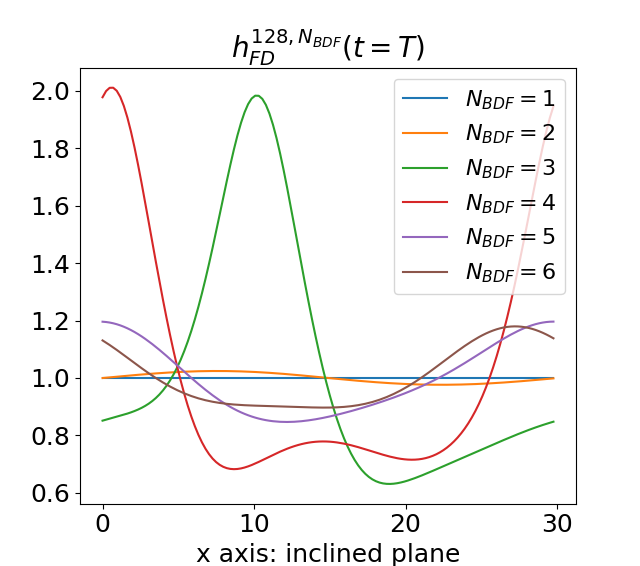
\includegraphics[width=\textwidth]{Verif_scheme/plot_FD_BDF_Nx_128.png}
        \caption{$N_x = 128$}
        \label{fig:image1}
    \end{minipage}
    \hfill
    % Second image
    \begin{minipage}[b]{0.45\textwidth}
        \centering
        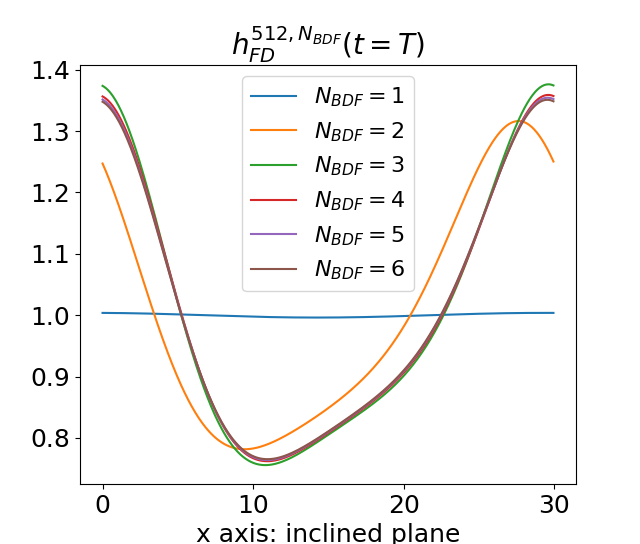
\includegraphics[width=\textwidth]{Verif_scheme/plot_FD_BDF_Nx_512.png}
        \caption{$N_x=512$}
        \label{fig:image2}
    \end{minipage}
    \caption{Plot at the final time of solutions computed with  several BDF Schemes from 1 to 6, and fixed space step. The case $N_x=128$ gives very different solution for different $N_{BDF}$ whereas we can make out a common behaviour among the schemes for the case $N_x512.$  }
    \label{fig:BDF_plot_128_512}
\end{figure}

\begin{figure}[h]
\centering
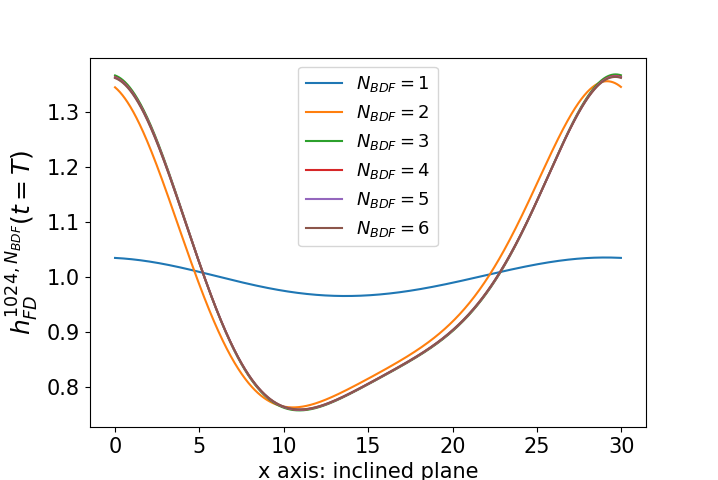
\includegraphics[width=0.75\textwidth]{Verif_scheme/plot_FD_BDF_Nx_1024.png}
\caption{We observe that the third, fourth, fifth and sixth order BDF schemes are quite close for $N_x = 1024.$ The second order is still quite difference while the first order solution doesn't have the same crest amplitude at all. }
\label{fig:BDF_plot_1024}
\end{figure}


We don't take risk and prefer to keep a high order. Therefore, for the control experiments that we will carry on later, we choose to take 
\begin{equation}
\boxed{
    N_x=512
    },
\end{equation}
as $N_x=1024$ is quite long to compute ( 1200s for the spectral scheme and 10000s for the Finite Difference scheme). We will choose $N_{BDF}$ with the next study of the convergence of the schemes.

\textbf{Convergence study of the schemes}
We compute $h^{(N_x, N_{BDF})}$ for different time steps and compare in $L^2$ and $L^{\infty}$ difference to the methods at the final time. We set the maximum number of points as $$N_x^{max} = 1024.$$ We take that specific number because it was high enough to have good results and can be divided $\{128, 256, 512\}$ so we won't need to make any interpolation when we do the difference between the arrays (which don't have the same shape).
 
So what we compute is 
\begin{equation}\label{h_diff_convergence_rate}
    ||h^{(N_x^{max}, 2)}(T)-h^{(n, 2)}(T)||_{L^{p}([0,L])}
\end{equation}
with $p\in \{2, +\infty\},n\in \{1024/i, i\in \{2, 4, 8\}\} = \{512, 256, 128\}.$
We test with the settings \eqref{eq_value_variables_num_verif} which give an exponentially growing regimes. The fact that the system forms an exponentially growing wave allows us to probably have all the discrepancy during the transitional regime amplified at the final time. Therefore, it justifies in a sense why we test the numerical scheme this way\footnote{We test exponentially growing regimes so differences during the transitional regime would be probably amplified at the final time.}.
\\

Among the $12=6\times2$ graphs (one for each methods and for each $N_{BDF}$) that we computed, we find that difference in $L^2$ and $L^{\infty}$ norm are decreasing exponentially, with a higher rate at $N_{BDF}=3$ and $4$. We show in figure \eqref{fig:Convergence_plot_BDF_4_Sp} a plot of \eqref{h_diff_convergence_rate} for the spectral method with $N_{BDF}=4.$
\\

\begin{figure}
    \begin{center}
        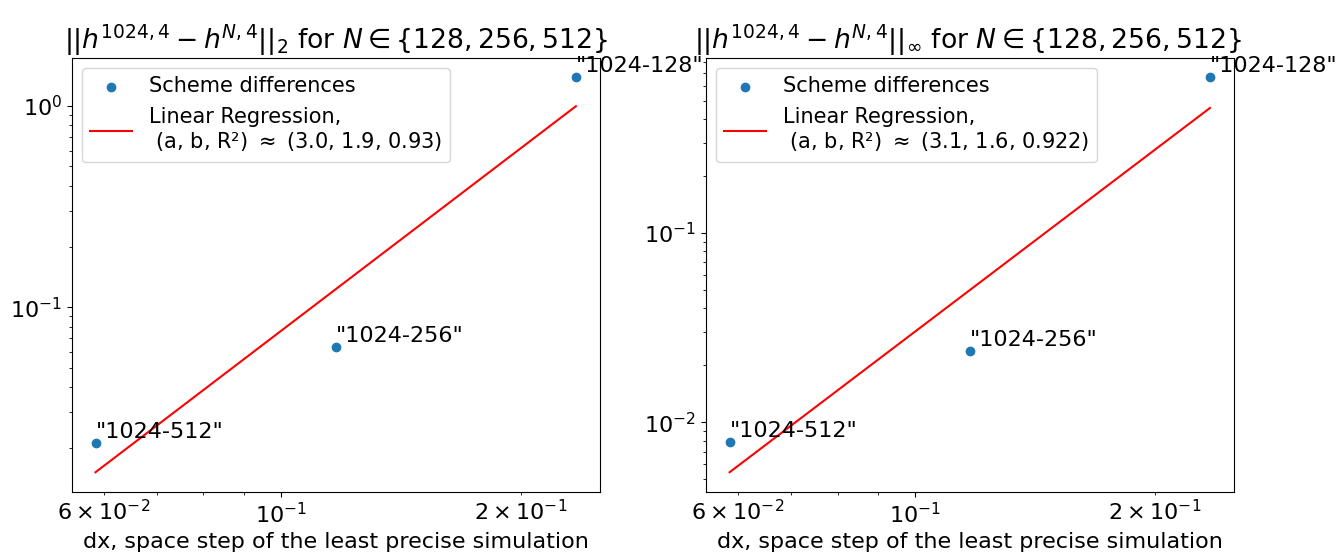
\includegraphics[width=\linewidth]{Verif_scheme/Convergence_graph_Sp_method.png}
    \end{center}
    \caption{Spectral method, $N_{BDF}=4$: Convergence plot at t=T in a log-log plot. }
    \label{fig:Convergence_plot_BDF_4_Sp}
\end{figure}

Taking into account the above observation and the one before, we choose 
\begin{equation}\label{var_final_config_tests}
\boxed{
    N_{BDF} = 4, \quad N_x = 512
}
\end{equation}

for the experimentation in the upcoming control part.
\\


\textbf{Comparison of the schemes.} We also compared the finite difference and spectral scheme to check if they match. We obtain a good matching of the schemes, with increasingly small errors with smaller space steps dx for $N_{BDF} \geq 3.$. In figure $N_{BDF}=4$, we have the error at $N_x = 512$ between $10^{-2}$ and ${10^{-3}}$ which is very small compared to the final amplitude of the regime, which is of $3.10^{-1}$.

\begin{figure}
    \centering
    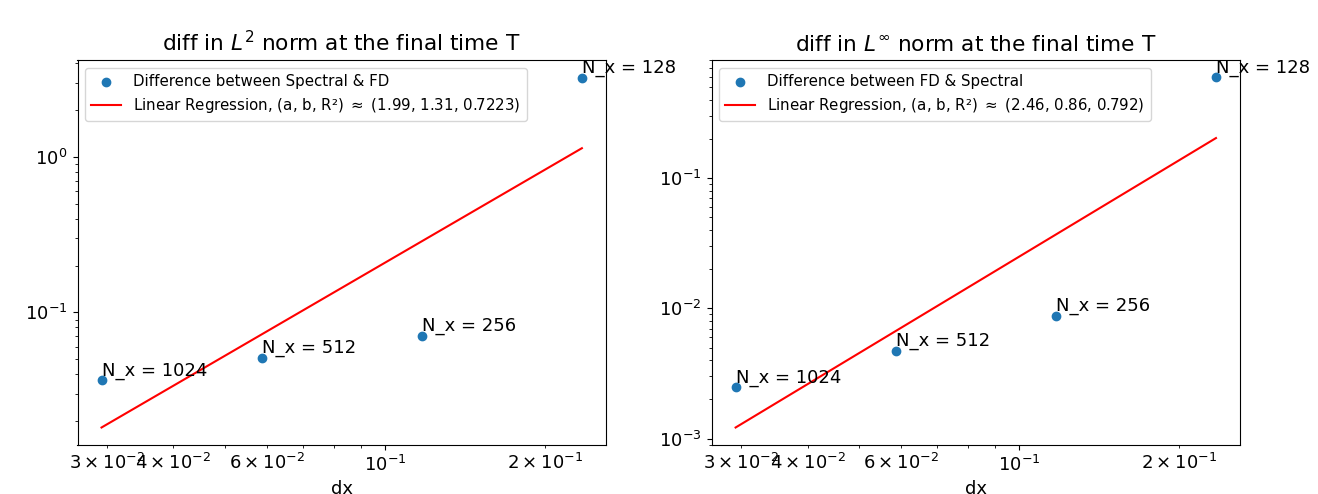
\includegraphics[width=1\linewidth]{Verif_scheme/Comparison_scheme_BDF4.png}
    \caption{Comparison between the Spectral and FD methods with $N_{BDF}=4.$ We see that the $L^{\infty}$ norm of the difference when $N_x=512$ is around $1.10^{-2}$ and $1.10^{-3}$ which is satisfactory for a final state of amplitude $3.10^{-1}$. }
    \label{fig:enter-label}
\end{figure}
\vspace{0.5cm}

\textbf{Physical properties.}
We check here some physical properties.
\\

The mass of the whole fluid is $M=\int_0^L\rho_l(x,t)h(x,t)dx$ and as $\rho_l(x,t)=\rho_l$ is uniform and static, we call "mass" the quantity 
\begin{equation}
M_h := \int_0^Lh = \frac{M}{\rho_l}.
\end{equation}

Integrating the Benney equation (\ref{Benney_ctrl_flux}), and deriving with respect to t, we have that: 
\begin{align*}
    M_{,t}&=\int_0^Lh_{,t}dx=-\int_0^L q_{,x}dx = -\int_0^L[q^B_{,x}+q^{control}_{,x}]dx \\ &= \int_0^L(h_{,x}h^2N_{s,x}+\frac{h^3}{3}N_{s,xx})dx=\int_0^L[\frac{h^3}{3}N_{s,x}]_{,x}dx ,
\end{align*}

where we used the Benney equation to introduce the flux q. We decomposed q into the Benney part (without the $N_s$) and control part : $(q^B, q^{control})$ and we supposed that the Benney equation without Control conserves mass, which is the case, numerically at least.
Finally, as h is L-periodic: 
\begin{equation}\label{mass_variation}
M_{,t} = \frac{h^3(0,t)}{3}(N_{s,x}(L)-N_{s,x}(0)).
\end{equation}
Therefore, the mass variation depends on the discontinuity gap of the derivative. 
We check this equality numerically by using actuators of the form $$N_s: x\in [0,L] \rightarrow \sum_{j=1}^{k}u_j(t)d(x-x_j),$$ with k being the number of air jets and d a gaussian with a significant standard deviation (i.e quite diffused), and we indeed see the height change according to the analytical rate with very small relative error ($\approx 1\%$ of the analytical rate \eqref{mass_variation}).  
\\

We also checked other qualitative properties. For example, if we put a higher air jet intensity, we will have deeper trough, or, for the same intensity, if we increase the slope angle $\theta$, we will have a bigger bump. We also played a bit with the viscosity and surface tension coefficient $\mu_l$ and $\gamma$.




%%%%%%%%%%%%%%%%%%%%%%%%%%%%%%%%%%%%%%%%%%%%%%%%%

\newpage
\section{Control}\label{Section_Control}
We use the linearized Benney equation (\ref{Benney_ctrl_linearised}) in order to use different type of control to stabilize the film height towards the Nusselt solution. We will present proportional control and state Feedback Linear Quadratic Regulator (LQR) Control strategies. Both strategies don't put any constraints on the sign of the control which has to be positive in our case (blowing air jets), so we also test if the positive part of these control can stabilize the film. Finally, none of these strategies ensure theoretically that the height and the control stay positive, i.e a positive control system. Hence, we construct an asymptotically stable positive control scheme and try to make it work numerically.  



\subsection{Continuous and discrete Control system }
In this section, we present the continuous and discrete linear control system with feedback control and link it to the falling liquid system that we study.

\subsubsection{The exponential system}
We want to stabilize the fluid towards the normalized Nusselt solution h(x,t) =1. To do that, we want to use a linear control strategy framework of the form

\begin{equation}\label{Ctrl_framework_continuous}
    \left\{ 
    \begin{aligned}
        x_{,t} = \mathcal{A}x+\mathcal{B}u, \quad y=\mathcal{C}x\\
        x(t=0) = x_0
    \end{aligned}
    \right.
\end{equation}
with $x, u, y\in L^{2}(\mathbb{R}_+, L^{\infty}([0,L],\mathbb{R}))$ the state of the system, the control, and the output (or observations) of the system respectively. $\mathcal{A}, \mathcal{B}$, and $\mathcal{C}$ are bounded linear operators that describe respectively the control-free dynamical system, the control impact on the system, and how much we can observe the state x.
\\ 

The discrete equivalent system which is more tractable for our numerical approach is 
\begin{equation}\label{Ctrl_framework_discrete}
    \left\{ 
    \begin{aligned}
        x_{,t} = Ax+Bu, \quad y=Cx\\
        x(t=0) = x_0
    \end{aligned}
    \right.
\end{equation}

with $\forall t\geq 0, x(t)\in \mathbb{R}^n$, $u(t)\in \mathbb{R}^k$, and $y(t) \in \mathbb{R}^n$, $A \in \mathcal{M}_{n}(\mathbb{R})$, $B \in \mathcal{M}_{n, k}(\mathbb{R})$, $C \in \mathcal{M}_{n}(\mathbb{R})$. Here, $n,k \in  \mathbb{N}^*$ are respectively the number of space discretization point for x and u, and number of actuators for u. \\

We chose to take 

\begin{equation}
    C = I_d
\end{equation}
which means that we have a \underline{ full observation of our state}, which is a strong assumption. Indeed, as we will see later in the next section (\ref{sub_section_link_ctr_FLF}), the state x will be the height of the film. Having full observation means that we can, at all time, measure exactly the height. These kind of assumptions can be realistic with laboratory equipment, like in (\cite{experimental_paper}) where they use precise optical measurements and vision algorithms to measure accurately the height of the liquid film. However, in an industrial framework, it is not sure that this hypothesis is still realistic. It becomes even more difficult in the case of the Weighted Residuals model, another reduced order model of the Navier-Stokes equations, as one would have to measure exactly the height h and the flux q. 
\\

As we want to use a feedback control strategy, the control is of the form 
\begin{equation}
    u = Ky = Kx, \quad K \in \mathcal{M}_{k,n}.
\end{equation}

Hence, the system can be rewritten as 
\begin{equation}\label{expo_ctrl_system}
    \left\{
    \begin{aligned}
        x_{,t}=(A+BK)x \\
        x(t=0) = x_0
    \end{aligned}
    \right.,
\end{equation}
which is an exponential system with solution $$s:t\mapsto  e^{(A+BK)t}x_0.$$

As we want the system to be stable, all the eigenvectors of the matrix A+BK have to have a negative real part so that their exponential vanish. We call these matrices \underline{Hurwitz matrices}. 
Therefore, the problem can be finally rewritten as a \underline{pole placement problem}: 
\begin{equation}\label{eq_pole_placement}
\boxed{
    \text{Find } K \in \mathcal{M}_{n,k},\quad \forall v \in Sp(A+BK), \mathfrak{R}(v) <0
    }
\end{equation}
or 
\begin{equation}\label{eq_pole_placement_Hurwitz}
    \text{Find } K \in \mathcal{M}_{n,k},\quad A+BK \text{ is Hurwitz,}
\end{equation}
with Sp the notation for spectrum and $\mathfrak{R}$ for the real part of a complex number.
\subsubsection{Link with the falling liquid system}\label{sub_section_link_ctr_FLF}
We link here the linear control framework with our physical system.. 

We take 
\begin{equation}
\tilde{h} = \frac{h-1}{\delta}
\end{equation}

the "zoomed" perturbation from the perturbed normalized height (\ref{h_linear_decomposition}). We recall linearized Benney equation with air jet control (\ref{Benney_ctrl_linearised}):
$$\tilde{h}_{,t} = \left[ -2\partial_x + (\frac{2cot(\theta)}{3}-\frac{8Re}{15})\partial_{xx} - \frac{1}{3Ca}\partial_{xxxx}\right]\tilde{h} + \left[ \frac{1}{3}\partial_{xx}\right]\tilde{N}_s.$$
\\

We take a (scaled) normal stress as a sum of k controlled actuators which represent the air jet: 
\begin{equation}
\boxed{
    \tilde{N}_s = \sum_{j=1}^ku_j(t)d(x-x_j),
}
\end{equation}
with 
\begin{equation}
    \forall x \in [0,L], \quad d(x)=Aexp\left(\frac{cos(\nu x)-1}{\omega^2}\right).
\end{equation}
A is here chosen such that $\int_0^Ld = 1$, $\nu=\frac{L}{2\pi}$ and $\omega$ to be chosen later in the program.\\


So the total equation becomes
\begin{equation*}
    \tilde{h}_{,t} = \mathcal{A}\tilde{h} + \mathcal{B} u
\end{equation*}
with
\begin{align*}
     u&=(u_j)_{j\in[|1,k|]}\in L^2(\mathbb{R}_+,\mathbb{R})^k, \\
     \mathcal{A}&= -2\partial_x + (\frac{2cot(\theta)}{3}-\frac{8Re}{15})\partial_{xx} - \frac{1}{3Ca}\partial_{xxxx},\\
\end{align*}
and 
\begin{equation*}
         \mathcal{B}: \left(
         \begin{aligned}
             u\ &\mapsto \left( t \rightarrow \frac{1}{3}\sum_{j=1}^ku_j(t)d_{xx}(.-x_j) \right) \\
             L^2(\mathbb{R}_+,\mathbb{R})^k &\rightarrow L^2(\mathbb{R}_+, L^{\infty}([0,L], \mathbb{R}))
         \end{aligned}
         \right).
\end{equation*}
We see the link with the continuous linear control model (\ref{Ctrl_framework_continuous}) with the same notations, except for the state x which is here $\tilde{h}$. We only have a little difference with the control u as we introduced a specific form for the control so the functional space is a bit different, but it will not affect the discrete problem. \\

 \textbf{The discrete system}
We discretise the system and have $N_x$ numbers of ODEs. We add also the feedback control with full observations: 

\begin{equation}\label{eq_discrete_ctrl_FLF}
\boxed{
\frac{d\tilde{h}}{dt} = A\tilde{h} + B u, \quad u = K\tilde{h}.}
 \end{equation}

We directly have the similarity with the discrete linear control framework (\ref{Ctrl_framework_discrete}) with $$n \approx N_x, x \approx \tilde{h} \in \mathbb{R}^{N_x}, A \in \mathcal{M}_{N_x}, B\in \mathcal{M}_{N_x, k} \text{, and }  C= I_d \in \mathcal{M}_{k, N_x}$$.

The matrices A and B are constructed with a centered finite difference scheme, so using the notations of the finite difference matrices, the matrix A is : 

\begin{equation}
\boxed{
\begin{aligned}
    A &= \alpha_1 mat_{FDper}(N_x, (0, -1, 1))+\alpha_2 mat_{FDper}(N_x, (-2, 1, 1))\\
    &+ \alpha_3 mat_{FDper}(N_x, (6, -4, -4, 1, 1)), \\
\end{aligned}
}
\end{equation}


with $$\alpha_1 = \frac{-2}{2dx}, \alpha_2 = \frac{1}{dx^2}(\frac{2cot(\theta)}{3}-\frac{8Re}{15}), \alpha_3 = \frac{-1}{3Cadx^4}.$$
\\

The matrix B is 
\begin{equation}
    \boxed{
    B = (\frac{1}{3}d_{xx}(x_i-x_j))_{(i, j)\in[|1,N_x|]\times[|1, M|]} \in \mathcal{M}_{N_x, M}(\mathbb{R})
    }
\end{equation}
as $$ \forall i \in [|1, N_x|], \quad \sum_{j=1}^MB_{ij}u_j(t) = (B u(t))_i = (\frac{1}{3}\partial_{xx}N_s)_i = \frac{1}{3}\sum_{j=1}^M u_j(t)d_{xx}(x_i-x_j).$$


\subsection{LQR Control}
In this section, we implement Linear Quadratic Regulator (LQR) Control. As its name suggests it, it is a type of linear control linked to a quadratic function. This function will be here a cost that we will going to introduced further. We will see that LQR control succeeds to stabilize the Benney system. In the same spirit as the proportional control, we do blowing air jets only control by taking the positive part of the control at each time steps. Here again, we find that despite being less efficient then the classic LQR, the positive part of the LQR control stabilizes successfully the Benney system. 

\subsubsection{LQR Control and Riccati equation}
We first deal with the continuous system an introduce the cost function 

\begin{equation}
    \kappa(u) = \int_0^{+\infty}\int_0^L \left[\beta (\tilde{h}(t)-\xi(t))^2+ (1-\beta)\tilde{N}_s(x,t)^2\right]dxdt.
\end{equation}

It is a cost functional whose weight $\beta$ translates the importance given to the distance between the system state x to a goal state $\xi \in L^2(\mathbb{R}_+, L^2([0,L],\mathbb{R}))$ compared to the quadratic cost of the control. As we want to stabilize the system towards the Nusselt solution ($\tilde{h}=0)$, we take naturally $$\xi = 0.$$




Let us define $$D=(d(x_i-x_j))_{(i,j)\in [|1,N_x|]\times [|1,k|]}$$ with d the shape function of the air jet actuators. We then define the discrete counterpart of the continuous cost $\kappa$: 

\begin{equation}\label{eq_LQR_discrete_cost}
\boxed{
    c = \int_0^{+\infty}(\tilde{h}^TQ\tilde{h}+u^TRu)dt}
\end{equation}
with 
\begin{equation}\label{eq_LQR_discrete_cost_matrices}
   R=(1-\beta)\frac{L}{N_x}D^TD\quad \text{ and } \quad  Q=\beta \frac{L}{N_x}I_{N_x}.
\end{equation}

We justify this definition of c with the following approximations of integrals by their Riemann sums (rectangle method):

$$\beta\int_0^L\tilde{h}^2(x,t)dx \boxed{\approx} \frac{L}{N_x}\sum_{i=1}^{N_x}\tilde{h}^2(x_i,t) = \beta\frac{L}{N_x}\tilde{h}^T\tilde{h}=\tilde{h}^TQ\tilde{h}$$
and 
\begin{align*} (1-\beta)\int_0^L N_s^2(x, t)dx &= (1-\beta)\int_0^L(\sum_{j=1}^{M}u_j(t)d(x-x_j))^2dx \\ &\boxed{\approx} (1-\beta)\frac{L}{N_x}\sum_{i=1}^{N_x}(\sum_{j=1}^{M}u_j(t)d(x_i-x_j))^2 \\&= \sum_{1\leq j, k\leq M}u_j(t)u_k(t)((1-\beta)\frac{L}{N_x}\sum_{i=1}^{N_x}d(x_i-x_j)d(x_i-x_k)) \\ &= \sum_{1\leq j, k\leq M}u_j(t)u_k(t) R_{j,k} = U^TRU.\end{align*}



\textbf{The Riccati equation.}Now we present how we find the optimal control associated with the discrete cost c by solving a matrix equation. We know from \cite{A_Thompson_FLF_blowing_suction} (part 3.2) for example, that if find a symmetric positive semi-definite matrix P solution to the problem

\begin{equation}\label{eq_Riccati_eq}
    \text{Find } P\in \mathcal{M}_{N_x}, \quad 0=A^TP+PA+R-PBR^{-1}B^TP, 
\end{equation}

 we can build a gain matrix of this form:
 \begin{equation}
    K = -R^{-1}B^TP.
 \end{equation}
 
 The equation \eqref{eq_Riccati_eq} is known as the \underline{Continuous Algebraic Riccati Equation} (CARE). At the opposite of \cite{holroyd2023linearquadraticregulationcontrol}, we don't use a specific method to solve this equation and rather use the python library \textit{python-control} with the function \texttt{control.lqr}. We also didn't check the existence of a solution, but let us remark that in the continuous framework, if the system (A, B) is controlable,  R is positive definite and Q semi-positive definite, then there exists one and only minimizer of the cost functional $\kappa$ which solves the Riccati equation. Here, R and Q are obviously positive semi-definite and we will check numerically that R is positive definite. 


 % PUT FIGURE OF A GAIN MATRIX ROW
 
\subsubsection{Numerical experiment}
We now try to stabilize the growing regime \eqref{eq_value_variables_num_verif} with LQR
control. We test first classic LQR control, which stabilizes efficiently the system. Then,
we try to apply only the positive part of the LQR control, to mimic blowing only air jets.
We find that this control also stabilizes the system, but is less efficient. 
\\

\textbf{Classic LQR Control.} We implemment the LQR control by solving the Riccati equation, 
as described at the end of the previous section. We test several weight parameters $\beta
\in \{0.2, 0.5, 0.95 \}$\footnote{Let us precise that the program doesn't find a solution for
Riccati equation for some values of $\beta$ like 0.1 or 0.5. That is why we take here $\beta=0.2$
as a 'small' $\beta$.} to observe how this parameter affects the stabilization of the system,
but also the total quadratic cost of the control. Here, we don't take into account the shape functions
 of the actuators and just look at the their amplitudes as we just want to compare the cost obtained 
 with different values of $\beta$.: 
\begin{equation}
    \kappa_u = \int_{0}^{T} \int_{0}^{L}u^2 dx dt,
\end{equation}

or rather its numerical counterpart:

\begin{verbatim}
    quad_cost_ctrl = np.sum(amplitudes_spectral**2)*dx**2*dt**2.
\end{verbatim}

Here, \textit{"amplitudes\_spectral"} the amplitudes of the shape function with a spectral method 
numerical scheme.  
\\

We consider that the system is stabilized when its maximal amplitude is lower than $\delta=1$, the 
amplitude of the initial perturbation. We take 


\begin{equation}
    T_{start} = 160, \quad T=300
\end{equation}

the starting time of the control (to let the perturbation grow until a sufficient large state) and
the total time of the simulation to let the time to the control to stabilize the system.
The control stabilizes exponentially the system, as we can see in figure \eqref{fig:LQR_beta_0.95}.We 
present in \eqref{tab:LQR_cost_beta} the cost for different $\beta$.


\begin{figure}
    \centering
    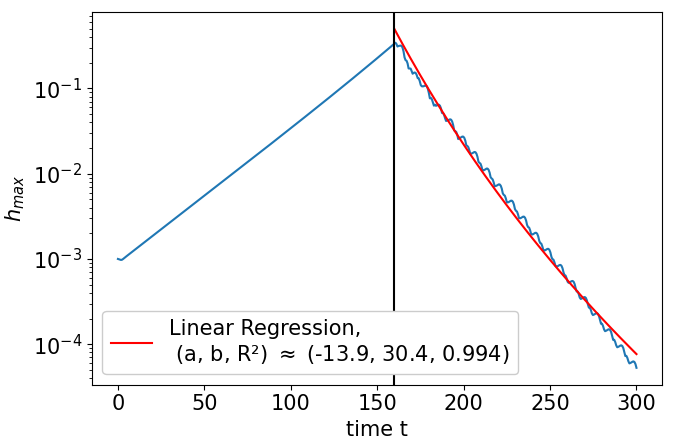
\includegraphics[width=0.5\linewidth]{Control_experiments/LQR_beta_0.95.png}
    \caption{Stabilization of the Benney system with an LQR control of parameter $\beta=0.95$.
    We made an exponential regression (so linear in a log scale) to see the scale of dampening.
    Let us stress out that the decrease rate is with respect to the classic neperian logarithm
    while the log scale in this plot is with respect to the logarithm in base 10. Therefore,
    the slope angle doesn't match with what we see in the plot (need to rescale it with log(10)) }
    \label{fig:LQR_beta_0.95}
\end{figure}
\vspace{0.5cm}


\begin{table}[ht]
    \caption{Array of the cost with different values of $\beta$}
    \label{tab:LQR_cost_beta}
    \centering
        \begin{tabular}{ |c|c|c|c| }
        \hline
             $\beta$ & 0.95 & 0.5 & 0.2  \\
        \hline
        $\kappa_u$ & 3.2744 & 3.03386 & 3.0285 \\ 

        \hline
        \end{tabular}
\end{table}

We see that $\kappa_u$ is increasing with $\beta$, which is expected as we lower the weight
on the cost of the control to have a better stabilization.\\

The LQR control stabilizes well the Benney system, and the videos of the 3 controls can be seen in the 
\href{https://github.com/Bilal59170/Repo_Warwick_internship}{Github repository}. As said before, 
this result is not sufficient as it gives not only blowing, but also suction air control. 
\\


\textbf{Positive part of LQR Control.}
Now, we only take the positive part of the LQR control too construct a blowing only air jet control.
We find that the system stabilizes also exponentially but around 3-4 times slower, with the coefficient 
of the exponential regression bein around 3 in the positive part case against 14 in the normal case. We 
tried to carry out simulations with T = 1000 in order to see the decrease of the amplitude until the
end. However, the configuration given by \eqref{var_final_config_tests} doesn't seem to be enough as the 
system Benney system with variables \eqref{eq_value_variables_num_verif} blocks before t=160 (the time on when
the system wasn't blocking with $N_x =512$ and $N_x=1024$), which seems to mean that the number of 
time (here $N_t = N_x = 512$) and steps point isn't enough for T=1000. 

From a physical point of vue, it was expected that the control will be less efficient as we remove half 
of the energy of the normal LQR control. 


\subsection{Proportional Control}
We want now to compare the LQR result with proportionnal control. Indeed, we saw in the videos of the dynamics 
of the liquid film height that the actuators seemed to have a behavior very close to the one of proportionnal 
control (sucking when there is a trough, blowing when there is a crest). Therefore, we lean on proportionnal control,
a simpler control mechanims, to see if the complexity of the LQR was necessary to have good results.

We now do proportional control i.e control of the type 
\begin{equation}\label{N_s_prop_ctrl}
    \tilde{N}_s = \alpha\tilde{h} = \alpha \frac{h-1}{\delta}, \quad \alpha >0.
\end{equation}

Physically, $\tilde{N}_s >0$ when there is a crest i.e when $\tilde{h}>0$, so we push when there is a crest and suck when there is a trough which is quite a basic and intuitive think to do to flatten the fluid. 
\\

 We do exactly the same type of analysis as \cite{Thompson_2016_prop_ctrl} where they did proportional control with fluid blowing and suction actuation. To find a criterion on $\alpha$, we make a stability analysis on linearized Benney equation \eqref{Benney_ctrl_linearised} and take the feedback form of $\tilde{N}_s$ \eqref{N_s_prop_ctrl}:  

\begin{equation}
\tilde{h}_{,t} = \left[ -2\partial_x + \left( \frac{8}{15}(Re_0-Re)+\frac{\alpha}{3}\right)\partial_{xx} - \frac{1}{3Ca}\partial_{xxxx}\right]\tilde{h} 
\end{equation}

So, similarly to \eqref{subsubsection_linear_theory} the dispersion relation becomes

\begin{equation}\label{eq_dispertion_prop_ctrl}
    \forall k\in \mathbb{N},\quad \lambda_k = -2ik+ k^2\left(\frac{8}{15}(Re-Re_0)-\frac{\alpha}{3}-\frac{k^2}{3Ca}\right).
\end{equation}

To stabilize the system in the linear approximation for any type of perturbations, we want $$\forall k \in \mathbb{N}^*, \mathfrak{R}(\lambda_k) <0$$

which is equivalent (except for $k=0$) to take 
\begin{equation}
    \alpha > \alpha_{AJ}= \frac{24}{15}(Re-Re_0).
\end{equation}


In comparison, the coefficient $\alpha$ for blowing and suction in paper \cite{Thompson_2016_prop_ctrl} was 
\begin{equation}
    \alpha_{BS} = \frac{16Ca(Re-Re_0)^2}{75}.
\end{equation}

We see that $\alpha_{AJ}$ doesn't depend on the capillary number depends linearly on $(Re-Re_0)$, while $\alpha_{BS}$ depends linearly on Ca and quadratically on $(Re-Re_0)$. Physically speaking, is it surprising that the Capillary number appears in the blowing and suction mechanism but not in the air jets one as the air jet interact directly with the liquid surface. Mathematically speaking, we remark that any proportional control which affects only the second derivative will not depend on Ca \footnote{Only a control on the even derivative will have an effect in the amplitude in this linear theory, whereas the control on the odd derivative could act on the speed of the wave (the imaginary part of $\lambda_k$). Maybe that a control on the 4th derivative could be better than the air jet or blowing and suction one.}. Let us now evaluate these coefficient with the value that we used with the numerical scheme verification \eqref{eq_value_variables_num_verif}. We have 

$$\alpha_{AJ} = \frac{24}{15}(5-0.72) = 6.9, \quad \alpha_{BS} = \frac{16\times 1.10^{-3}}{75}(5-0.72)^2= 0.0039.$$

The blowing and suction actuation seem to be far more


% \begin{figure}[h]
% \includegraphics[width=1\textwidth]{}
% \caption{Plots of the $\mathfrak{R}(\lambda(k))$ with $\alpha = 0$ and $\alpha = \alpha_{AJ} $ in the left plot, and $\alpha = 0$ and $\alpha = \alpha_{BS}$ in the right plot. We can see that while the curve is just shifted down the y-axis in the blowing and suction case, its curvature is changed in the air jet case. It is expected as the $\alpha$ coefficient appears as a second order term (i.e in $k^2$) so it has an influence on the second derivative of $\mathfrak{R}(\lambda(k))$, so on its curvature.}
% \label{fig:prop_ctrl_dispersion}
% \end{figure}

In the blowing and suction case,  the coefficient $\alpha_{AJ}$ is the maximal coefficient where there exists a mode $k$ sucht that $\mathfrak{R}(\lambda(k)) \geq 0.$. For an $\alpha$ above that threshold, all the modes are exponentially decreasing and the solution flattens towards the Nusselt solution. It is not the case of the air jet actuation method where we will always have $\lambda_0=0.$ Indeed, a non zero order 0 mode would imply having a different mass as the one of the Nusselt solution as we add something whose average is different than zero. Therefore, it was expected that $\lambda_0 = 0$ because the air jet actuation conserves the mass of the liquid so its mean height will not change. We can see in \eqref{fig:prop_ctrl_dispersion} that the control changes the curve of the dispersion relation but not its value on $k=0$.
\\

In both air jet and blowing/suction cases, the $\alpha$ coefficient is not enough to stabilize the real discrete system. Indeed, this coefficient was built with the assumption that we have actuators on all the points of the continuous domain (called "distributed control" in \cite{Thompson_2016_prop_ctrl}). However, this is not the case a continuous actuation is not possible (at least to the author's knowledge) and we want to have few actuators ( around 5) so that it can be convenient for industrial purposes. 

Therefore, we go back to the discrete system that we set in the previous section \eqref{eq_discrete_ctrl_FLF}. The idea of proportional control is that all actuators have the same proportional answer $\alpha$ to the height. Therefore, the gain matrix is here 
\begin{equation}
    K = \alpha I_{k, N_x} \in \mathcal{M}_{k,N_x}
\end{equation}

Hence, the poll placement problem \eqref{eq_pole_placement} becomes: 


\begin{equation}\label{eq_pole_placement}
\boxed{
    \text{Find }\alpha \in \mathbb{R}_+,  \quad \forall v \in Sp(A+\alpha BI_{k, N_x}), \mathfrak{R}(v) <0
    }
\end{equation}



\subsection{Positive control system}
We saw that we could stabilize the system with blowing-only air jets. We constructed the proportional and LQR control from the linear theory with a space and time continuum (i.e no discretization) so these methods are backed with analytical results. However, we don't have any theoretical backup for the positive controls that we built by taking the positive part of the proportional and LQR controls. In this section, we try to find a gain matrix that would keep the control positive and make the Benney system asymptotically stable. We find a system of linear inequalities that would give the wanted solution. We try to solve it numerically by reformulating it as a classic QP (Quadratic Programming) optimization problem.


\subsubsection{Positive control system}

We want to build a control in a way that we can prove analytically that the hight will stay positive and the control too. First, we reformulate the linear control system \eqref{eq_discrete_ctrl_FLF} using the initial height $h = 1 + \delta \tilde{h}$:

\begin{align}
    \frac{dh}{dt} &= \delta\frac{d\tilde{h}}{dt} = \delta \left[ A\tilde{h} + Bu\right] \\
    &\stackrel{(\tilde{h}=\frac{h-1}{\delta})}{=} Ah + \delta Bu - A \begin{pmatrix}
        1 \\ \vdots \\ 1
    \end{pmatrix} .
\end{align}

As A is a derivation matrix, 
$A \begin{pmatrix}
        1 \\ \vdots \\ 1
\end{pmatrix} =0$, so we have the new control system

\begin{equation}\label{pos_ctrl_system}
\left\{
\begin{aligned}
    &\frac{dh}{dt} = Ah+Bu = (A+BK)h\\
    &h(t=0) = h_0
\end{aligned}
\right. 
\end{equation}
\\

It gives again an exponential system of matrix A+KB. The difference with the problem \eqref{expo_ctrl_system} is that we have here a sign constraint on h and u since they have to stay positive, so just having A+KB being a Hurwitz matrix is not sufficient. Let us then define the notion of positive system.
\\

\underline{\textit{Definition and theorem:} Positive system and Metzler matrix}

Let $A \in \mathcal{M}_n.$ The exponential system 

\begin{equation}
\left\{
\begin{aligned}
\frac{dh}{dt}&= Ah\\
h(0) &= h_0 
\end{aligned}
\right.
\end{equation}

is said to be \underline{positive} according to \cite{pos_ctrl_paper}, if 
\begin{equation}
    h_0 \in \mathbb{R}_+ \implies \forall t \geq 0, h(t) \geq 0.
\end{equation}
Furthermore, the system is asymptotically stable if and only if 

\begin{equation*}
    \forall (i,j) \in [|1,n|]^2, i\neq j \implies A_{i,j} \geq 0.
\end{equation*}
This type of matrix are called \underline{Metzler matrix}
\\

Therefore, to have a positive and asymptotically stable system, we would need that A+KB is a Hurwitz and Metzler matrix. 

To ensure that the control is also positive, \cite{pos_ctrl_paper} gives a way to build the gain matrix K by solving this system of linear inequalities: 


\begin{equation}\label{linear_inequalities_pos_ctrl}
\text{Find } d\in \mathbb{R}^n,(z_j)_{1\leq j \leq n}\in (\mathbb{R}^k)^n, \quad \\
    \left\{ 
\begin{aligned}
&Ad+\delta B\sum_{i=1}^n z_i <0 \\
&d>0\\
&z_i \geq 0 \quad \forall i \in  [|1,n|]\\
&a_{ij}d_j + \delta b_j^Tz_j\geq 0 \quad \forall i\neq j 
\end{aligned}
\right. .
\end{equation}

The gain matrix is finally given by 
\begin{equation}
\boxed{
    K = (d_1^{-1}z_1| \dots |d_n^{-1}z_n).
}
\end{equation}

Here, according to the paper, the first and inequalities ensure that $A+\delta BK$ is Hurwitz, the last that it is Metzler, and the third that the control will be positive as the gain matrix will have non negative coefficient. Indeed, if $A+\delta BK$ is Metzler and Hurwitz, the system \eqref{pos_ctrl_system} is positive and asymptotically stable. Therefore, as the state of the system is non negative, the feedback control will also be non negative. 

\subsubsection{Reformulation into a QP optimization problem}
As we don't find any solver for linear inequalities system , we reformulate  \eqref{linear_inequalities_pos_ctrl} as a constrained Quadratic Programming Optimization problem.
\\

First, we construct the matrices $H \in \mathcal{M}_{n,n+nk}$ and $M \in \mathcal{M}_{n^2,n+nk}$ which will translate the first (one of the two conditions for matrix to be Hurwitz) and last lines (the only condition for the matrix to be Metzler) of the system. 

 Let us set $$v=\begin{pmatrix}d\\ z_1 \\ \vdots \\ z_n
\end{pmatrix}.$$

Then, 
$$Ad + \delta B\sum_{i=1}^n z_i <0 \Leftrightarrow H
v
<0 \text{ with } \quad H = (A,\delta B,-,\delta B) \in \mathcal{M}_{n,n+nk}.$$

As of M, we take $s = (i-1)n + j \in [|1,n^2|]$ so that we characterise the couple $(i,j) \in [|1,n|]^2$ only with s by
$$i_s = 1+\lfloor\frac{s-1}{n}\rfloor, \quad j_s=(s-1)\%n+1.$$

Next, $$(a_{ij}d_j+\delta b_iz_j >0 \quad \forall i \neq j )\Leftrightarrow Mv > 0$$

with
$$M_{sr} = 
\left\{ \begin{aligned}
0 &\text{ if } i_s=j_s \\
a_{i_s j_s} &\text{ if } r=j_s\\
\delta b_{i_s,r-(n+(j_s-1)k)} &\text{ if } r\in [|n+(j_s-1)k+1, n+j_sk|]
\end{aligned}\right. .$$
\\

Finally, we call $$v_{tot} = \begin{pmatrix}v\\v\end{pmatrix}.$$
The Metzler and Hurwitz conditions are then : $$Gv_{tot} <0, \quad \text{with }G = \begin{pmatrix}-M\quad 0 \\ 0 \quad H\end{pmatrix}.$$Then, we enforce that $v_{tot, c} = v_{tot, c+n+nk}$ (i.e that $v_{tot} = \begin{pmatrix}v\\v\end{pmatrix}$) with: $$A_{QP}v_{tot} = 0_{n+nk},\quad \text{with } A_{QP}= (Id_{n+nk},-Id_{n+nk}).$$


Finally we have this Optimization problem: 
\begin{equation}\label{opti_problem_pos_ctrl}
\begin{aligned}
\min_{v_{tot}\in \mathbb{R}^{2(n+nk)}}\quad &v_{tot}^TSv_{tot}\\
s.t \quad &Gv_{tot} <h:=0\in\mathbb{R}^{n^2+n} \\
&A_{QP}v_{tot}= b:=0 \in \mathbb{R}^{n+nk}\\
&v_{tot} > lb:=0 \in \mathbb{R}^{2(n+nk)}
\end{aligned}    
\end{equation}

with S such that we minimize the $(z_i)_{i\in[|1,N_x|]}$ to have a small cost for the control as the gain matrix would have small component.\\


\textbf{Numerical Solving.} To solve \eqref{opti_problem_pos_ctrl}, We use the python package \texttt{qpsolvers} that can be found in this \href{https://github.com/qpsolvers/qpsolvers}{Github repository}. 

We didn't succeed to find a solution which was Hurwitz and Metzler in the same time, even for small values of $N_x$. Concretely, the first part of the vector $v_{tot}$  outputed by the solver would encode a Hurwitz Matrix, while the second part would encode a Metzler matrix, but never both of the properties. Moreover, the solver would output very small values (around $10^{-14}$) with d being significantly smaller than the $(z_i)_{i\in[|1,N_x|]}$, so the control would be too large and make the numerical scheme bug. 




%%%%%%%%%%%%%%%%%%%%%%%%%%%%%%%%%%%%%%%%%%%%%%%%%
\newpage
\appendix
\section{The code}
\subsection{Scheme for the KS equation}\label{KS_computation_numerics}

We study the truncated system. In the code, we update the cosinus and sinus part separatly. Here, for convenience, we just detail the part for the cosinus update but the non linearities depends also on the sinus part.
\\
As the scheme needs the values of the Fourier modes for the first p time steps, we compute them with a classic implicit Euler scheme on the linearity, and explicit on the non-linearity. This starting scheme is exactly the scheme we use for $p_{BDF}=1.$

We make and abuse of notation by calling the discrete operators only for the cosinus parts of the fourier transform A and B. We also denote p instead of $p_{BDF}$ as the formulas are a bit heavy.

Therefore: 
$$AU^{d,n} = ((\lambda_j + \frac{1}{\nu})u_j^c(ndt)))_{1\leq j \leq M}, \quad B(U^{d,n}) = ((\frac{1}{\nu}u_j^c(ndt) + F_j^{d,c}))_{1\leq j \leq M}.$$


We denote $u^{c,n} =(u_j^c(ndt))_{j\in [|1,d|]}$
We call $\Lambda:= Diag(\lambda_1,\dots,\lambda_d)$ the diagonal matrix with $\lambda_j$,  so $$A = \Lambda + \frac{1}{\nu}I_d.$$
  
From the numerical scheme, we get that 
\begin{align*}
  (\alpha_p I_d + dtA)U^{d,n+p} = ((\alpha_p+\frac{dt}{\nu}) I_d + dt\Lambda)U^{d,n+p}\\
  = -\sum_{i=0}^{p-1}\alpha_iU^{d,n+i} + dt\sum_{i=0}^{p-1}\gamma_i B(U^{d,n+i}).
\end{align*}

So, only for the cosinus part:  
  
$$((\alpha_p+\frac{dt}{\nu}) I_d + dt\Lambda)u^{c,n+p}= -\sum_{i=0}^{p-1}\alpha_iu^{c,n+i} + dt\sum_{i=0}^{p-1}\gamma_i (\frac{1}{\nu} u^{c, n+i} + F^{d, c, n+i})$$

i.e 

$$u^{c, n+p}= ((\alpha_p+\frac{dt}{\nu}) I_d + dt\Lambda)^{-1}(-\sum_{i=0}^{p-1}\alpha_iu^{c, n+i} + dt\sum_{i=0}^{p-1}\gamma_i (\frac{1}{\nu} u^{c, n+i} + F^{d,c, n+i})) \in \mathbb{R}^d.$$

Finally, we "vectorize" the expression above. We introduce some matrices $\mathcal{U}^{d,c}$ and $\mathcal{F}^{d,c}$. Their row are for each time steps and their columns for each Fourier modes. We denote the extracted vector from $\mathcal{F}^{d,c}$ coordinate i to j included $\mathcal{F}_{i,j}^{d,c}$.


  $$H^{c, n+p}= ((\alpha_p+\frac{dt}{\nu}) I_d + dt\Lambda)^{-1}(-\underline{\alpha}_{p-1}^T.\mathcal{U}_{n, n+p-1}^{d,c}+ dt \underline{\gamma}_{p-1}^T.(\frac{1}{\nu} \mathcal{U}_{n, n+(p-1)}^{d,c} + \mathcal{F}_{n, n+(p-1)}^{d,c}) \in \mathbb{R}^d.$$

with  
$$\mathcal{U}_{n, n+(p-1)}^{d,c}, \mathcal{F}_{n, n+(p-1)}^{d,c} \in \mathcal{M}_{p-1, d},\quad \underline{\alpha}_{p-1} = (\alpha_0,..., \alpha_{p-1}) $$
and $$\underline{\gamma}_{p-1}= (\gamma_0, ..., \gamma_{p-1}).$$
\\ 

Which gives finally the expression of $u^s$ at the new time step:  
\begin{equation}
    \boxed{
    u^{c, n+p}= Diag((\frac{1}{\alpha_p+\frac{dt}{\nu} + dt\lambda_j})_{j\in [|1, d|]}) ((\frac{dt}{\nu} \underline{\gamma}_{p-1}^T-\underline{\alpha}_{p-1}^T).\mathcal{U}_{n, n+p-1}^{d,c}+ dt \underline{\gamma}_{p-1}^T.\mathcal{F}_{n, n+(p-1)}^{d, c}) \in \mathbb{R}^d.
    }
\end{equation}

Likewise (just changing the non-linearities),

\begin{equation}
    \boxed{
    u^{s, n+p}= Diag((\frac{1}{\alpha_p+\frac{dt}{\nu} + dt\lambda_j})_{j\in [|1, d|]}) ((\frac{dt}{\nu} \underline{\gamma}_{p-1}^T-\underline{\alpha}_{p-1}^T).\mathcal{U}_{n, n+p-1}^{d,s}+ dt \underline{\gamma}_{p-1}^T.\mathcal{F}_{n, n+(p-1)}^{d, s}) \in \mathbb{R}^d.
    }
\end{equation}

The 0th Fourier mode is taken null.Therefore, we have all the Fourier modes at time (n+p)dt.

\section{The governing equations}
The undimensionnalised Navier Stokes  equation \ref{eq NavierStokes1} are the Navier Stokes equation in the non-newtonian and incompressible case. 

\subsection{KBC and mass conservation}
The KBC is $$\frac{Df}{Dt}=\left[\frac{\partial}{\partial t}+(\underline{u}.\underline{\nabla})\right]f=0 \text{  with } f(x, y, z) = z-h(x, y, t).$$

So it gives $$h_{,t}=w-uh_{,x}-vh_{,y}.$$
$q_{x}(x,y,t)=\int_{0}^{h(x, y, t)}u(x, y, z,t)dz:=I_x(h(x, y, t), x,t)$\\
$q_y(x, y, t)= \int_{0}^{h(x, y, t)}v(x, y, z,t)dz:=I_y(h(x, y, t), x,t)$\\

So, as u(z=0) = v(z=0) = 0 (No slip),

$q_{x,x}=h_{,x}\partial_1I_x+1\times\partial_2Ix+0= h_{,x}[u(x, y,h,t)-0] + \int_{0}^h u_{,x}(x, u, z, t)dz$\\
$q_{y,y}=h_{,y}\partial_1I_y+1\times\partial_2Iy+0= h_{,y}[v(x, y,h,t)-0] + \int_{0}^h v_{,y}(x, u, z, t)dz$

So $$\underline{\nabla}.\underline{q}=h_{,x}u+h_{,y}v+\int_{0}^h(u_{,x}+v_{,y})dz.$$

Finally (KBC + Incompressibility),
$\underline{\nabla}.\underline{q}=w-h_{,t} - \int_{0}^h w_{,z}dz = w-h_{,t}-(w(x, y, h, t) - 0)$ so $$h_{,t}+\underline{\nabla}.\underline{q}=0.$$
\subsection{Dynamic boundary conditions}
Let us proove the Dynamic Boundary Conditions \ref{eq DBC1_Normal} and \ref{eq DBC_Tangential} in the 3D case and then return to the 2D one:

According to Kaliadasis book: 

\begin{equation}\label{eq DBC Kaliadasis}(\underline{\underline{\sigma_l}}-\underline{\underline{\sigma_g}}).\underline{n}=\gamma\kappa\underline{n}
\end{equation}

with $\kappa = \underline{\nabla}.\underline{n}$ and $\underline{n}=\frac{1}{\sqrt{1+h_{,x}^2+h_{,y}^2}}(-h_{,x}, -h_{,y}, 1)$ the normal points\underline{the gas from the liquid} which is the convention we're using in this document. Let's be carefull about that convention and somme potential sign errors as some paper takes the other direction (i.e gas->liquid) for the normal.

Hence, with the notation we have introduced in the paper, $$\underline{\underline{\sigma_l}}.\underline{n}+\underline{s_g}=\gamma\kappa\underline{n}.$$

We define $$N_s = \underline{s_g}.\underline{n}, \quad T_{si}=\underline{s_g}.\underline{t_i}, i\in\{x, y\}$$ with 

$$\underline{t_x}=\frac{1}{\sqrt{1+h_{,x}^2}}(1, 0, h_{,x}),\quad \underline{t_y}=\frac{1}{\sqrt{1+h_{,y}^2}}(0, 1, h_{,y})$$ 
$(\underline{n}, \underline{t_x}, \underline{t_y})$ is normalized, orthogonal and direct (simple computation). The convention taken in Radu's paper are the same but with a different direction of \underline{n} so it wasn't direct in that case.
\newline
\\
\\
\ref{eq DBC Kaliadasis}.\underline{n} gives:


\begin{align*}
\gamma \kappa |\underline{n}|^2&= \underline{n}.\underline{\underline{\sigma_l}}.\underline{n} + \underline{n}.\underline{s_g} \\
 &= \underline{n}.\left( -p_l \underline{\underline{I}} + \mu_l(\underline{\underline{\nabla}}^Tu_l+\underline{\underline{\nabla}}u_l)\right).\underline{n}+N_s\\
 &\overset{(u_l=u_g \text{ at } y=h)}{=} \frac{1}{1+h_{,x}^2+h_{,y}^2}(-h_{,x}, -h_{,y}, 1)\left[ -p_l\underline{\underline{I}} + \mu_l\begin{pmatrix}
2u_{,x} & u_{,y}+v_{,x} & u_{,z}+w_{,x} \\
\cdot & 2v_{,y} & v_{,z}+w_{,y} \\
\cdot & \cdot & w_{,z}
\end{pmatrix} \right](-h_{,x}, -h_{,y}, 1)^T\\ 
&+N_s
\end{align*}

And (cf Kaliadasis' book): 

$$\gamma \kappa |\underline{n}|^2 = \gamma \kappa = \frac{\gamma}{(1+h_{,y}^2+h_{,x}^2)^{3/2}}\left[ h_{,yy}(1+h_{,x}^2)+h_{,xx}(1+h_{,y}^2)-2h_{,y}h_{,x}h_{,yx}\right].$$

Hence (after non dimensionnalisation...)

$$\frac{\mu_lU_l}{h_l}\left[-p_l+\frac{2}{1+h_{,x}^2+h_{,y}^2}[\dots]+N_s\right]=\frac{\gamma}{h_l}\frac{1}{(1+h_{,y}^2+h_{,x}^2)^{3/2}}[\dots]$$

which gives finally, in 3D:

\begin{equation}
\begin{aligned}
-p_l &+\frac{2}{1+h_{,x}^2+h_{,y}^2}[h_{,x}^2u_x+h_{,y}^2+h_{,y}^2v_y+w_{,z}+h_{,x}h_{,y}(v_{,x}+u_{,y})-h_{,x}(w_{,x}+u_{,z})-h_{,y}(w_{,y}+v_{,z})]\\
&+N_s =\frac{1}{Ca}\frac{1}{(1+h_{,y}^2+h_{,x}^2)^{3/2}}[h_{,yy}(1+h_{,x}^2)+h_{,xx}(1+h_{,y}^2)-2h_{,x}h_{,y}h_{,yx}].
\end{aligned}
\end{equation}

In 2D (x<->x, y<->z, and y ignored) we retrieve \ref{eq DBC_Normal Control} i.e:

$$-p_l + \frac{2}{1+{h_{,x}}^2}(u_{,x}{h_{,x}}^2 - h_{,x}(u_{,y} + v_{,x})+v_{,y}) = \frac{1}{Ca} \frac{h_{,xx}}{(1+{h_{,x}}^2)^{3/2}}-N_s.
$$


\textbf{Tangential Case}
\ref{eq DBC Kaliadasis}.$\underline{t_x}$ gives: 

$$\underline{t_x}.(\underline{\underline{\sigma_l}}+\underline{s_g}).\underline{n}= \underline{t_x}.\underline{\underline{\sigma_l}}.\underline{n}+T_{sx}=\gamma\kappa\underline{t_x}.\underline{n}=0 \quad \text{(orthogonal)}$$

\begin{align*}
0 = \frac{1}{\sqrt{1+h_{,x}^2+h_{,y}^2}\sqrt{1+h_{,x}^2}}(1, 0, h_{,x})\left[ -p_l\underline{\underline{I}} + \mu_l\begin{pmatrix}
2u_{,x} & u_{,y}+v_{,x} & u_{,z}+w_{,x} \\
\cdot & 2v_{,y} & v_{,z}+w_{,y} \\
\cdot & \cdot & w_{,z}
\end{pmatrix} \right](-h_{,x}, -h_{,y}, 1)^T+T_{sx}
\end{align*}

So (undimensionnalisation \& computation..)


\begin{align*}
    \frac{1}{\sqrt{1+h_{,x}^2+h_{,y}^2}\sqrt{1+h_{,x}^2}} &\Big[
        2h_{,x}(w_{,z}-u_{,x})-h_{,y}(u_{,y}+v_{,x})\\
    &+(1-h_{,x}^2)(u_{,z}+w_{,x}) -h_{,x}h_{,y}(v_{,z}+w_{,y}) \Big]
    = -T_{sx}.
\end{align*}


Hence, in 2D, we retrieve the tangential part of \eqref{eq DBC_Control} i.e: 

$$    \frac{(v_{,x} + u_{,y})(1-{h_{,x}}^2)+2h_{,x}(v_{,y}-u_{,x})}{1+h_{,x}^2}= -T_s. $$

It's the same for $-T_{sy}$ with some indices swapping. Let us underline that the choice of the direction of $\underline{n}$ can change the $\pm$ before the $T_{sx}$ if we do not always take an direct orthonormal triplet $(N_s, T_{sx}, T_{sy})$. It's thus important to watch out to the significance these quantities (what does that mean if it's >0, <0). 

\section{Derivation of the reduced order models}
\subsection{Benney equation}
We present here only the scaling and the difference between the uncontrolled and the normal external pressure controlled cases. For more details, see the paper of "Falling liquid films with blowing and suction" from Alice.T and al. or the calculus on paper that I made. 

The chosen scaling is $$X=\epsilon x, \quad T=\epsilon t, \quad v=\epsilon w, \quad Ca=\epsilon^2 \hat{Ca}.$$

The order 0 for the pressure are given by the y-axis projection of the NS equation and the tangential KBC. We take $Ca=O(\epsilon^2)$ and $N_s$ of the same order as the liquid pressure $p_l$ so that surface and external pressure effects appears in the order 0 pressure of the liquid. In the 0-order pressure is given by $$p_{l0} = N_s+2(h-y)cot(\theta)-\frac{h_{,XX}}{\hat{Ca}}$$ with the scaled variables. The case without airjets is when $N_s=0$.

\subsection{The KS equation}

\printbibliography
\end{document}